\documentclass[12pt]{article}
\usepackage[margin=1in]{geometry}
\usepackage{amsmath,amssymb,amsthm,mathtools}
\usepackage{booktabs,threeparttable,setspace,enumitem,array,longtable,graphicx}
\usepackage[authoryear,round]{natbib}
\usepackage[colorlinks=true,linkcolor=blue!50!black,citecolor=blue!50!black,urlcolor=blue!50!black]{hyperref}
\usepackage{xcolor}
\onehalfspacing
\emergencystretch=2em

\newtheorem{theorem}{Theorem}
\newtheorem{proposition}[theorem]{Proposition}
\newtheorem{corollary}[theorem]{Corollary}
\newtheorem{lemma}[theorem]{Lemma}
\theoremstyle{definition}
\newtheorem{definition}[theorem]{Definition}
\newtheorem{assumption}[theorem]{Assumption}
\theoremstyle{remark}
\newtheorem{remark}[theorem]{Remark}
\newcommand{\R}{\mathbb{R}}
\newcommand{\E}{\mathbb{E}}

% Every empirical number below is generated from a committed result file by the thesis pipeline
% (thesis/checks/*.tex) or, for the exploratory robustness section, by robustness.py in this folder.
\makeatletter\def\input@path{{./}{../../../thesis/}}\makeatother
\input{checks/E1v2_numbers}\input{checks/D1_numbers}\input{checks/G1_numbers}\input{checks/V1_numbers}
\input{checks/C2_numbers}\input{checks/O1_numbers}\input{checks/C3_numbers}\input{checks/F1_numbers}
\input{checks/S1_numbers}\input{checks/R1_numbers}\input{checks/results_extra}% generated by robustness.py (exploratory); do not edit
\newcommand{\RobSBaseT}{4.82}\newcommand{\RobSBaseC}{-1.57}
\newcommand{\RobSWeekT}{3.75}\newcommand{\RobSWeekC}{-1.57}
\newcommand{\RobSSymT}{5.10}\newcommand{\RobSSymC}{-1.57}
\newcommand{\RobSTrFiftyT}{4.39}\newcommand{\RobSTrFiftyC}{-2.69}
\newcommand{\RobSTrSeventyT}{4.38}\newcommand{\RobSTrSeventyC}{-1.51}
\newcommand{\RobSWinsT}{5.52}\newcommand{\RobSWinsC}{-1.74}
\newcommand{\RobSYrAT}{2.32}\newcommand{\RobSYrAC}{-1.27}
\newcommand{\RobSYrBT}{4.15}\newcommand{\RobSYrBC}{-2.22}
\newcommand{\RobSNoOctT}{4.33}\newcommand{\RobSNoOctC}{-0.95}
\newcommand{\RobSHiVolT}{4.84}\newcommand{\RobSHiVolC}{-1.76}
\newcommand{\RobSLoVolT}{2.90}\newcommand{\RobSLoVolC}{-1.43}
\newcommand{\RobSLooMin}{4.40}\newcommand{\RobSLooMax}{5.37}
\newcommand{\RobRBaseE}{0.59}\newcommand{\RobRBaseSE}{0.09}
\newcommand{\RobRVolE}{0.29}\newcommand{\RobRVolSE}{0.15}
\newcommand{\RobRYrAE}{0.97}\newcommand{\RobRYrASE}{0.14}
\newcommand{\RobRYrBE}{0.08}\newcommand{\RobRYrBSE}{0.23}
\newcommand{\RobRKappaE}{0.70}\newcommand{\RobRKappaSE}{0.10}
\newcommand{\RobRSPsevenE}{-0.08}\newcommand{\RobRSPsevenSE}{0.04}
\newcommand{\RobRSShockE}{0.46}\newcommand{\RobRSShockSE}{0.12}
\newcommand{\RobRLooMin}{0.55}\newcommand{\RobRLooMax}{0.63}


\title{Identify or Certify?\\ What Public Market Data Reveal About Algorithmic Feedback}
\author{Pratik Niroula\thanks{Department of Computer Information Science, Minnesota State University, Mankato. \texttt{pratik.niroula@mnsu.edu}.}
\and Prashant Niroula\thanks{Faculty of Management, Tribhuvan University, Kirtipur, Nepal.}}
\date{Development revision, 30 October 2026. Author list to be settled with co-authors before circulation.}

\begin{document}
\maketitle

\begin{abstract}
\noindent Regulators ask to know which algorithms are trading. We ask which questions about those algorithms market data can answer, and at what cost. In a closed-loop model in which cohorts of algorithms respond to prices with exponential memory, every question an outside observer can ask is a functional of the merged measure of the cohorts' memory rates and weights. Identifying the cohorts is expensive: separating $K$ cohorts whose memory rates are $\Delta\eta$ apart needs a number of observations of order $(\Delta\eta)^{-(4K-2)}$, from experiments and from passive data alike. In the positive cohort class, certifying stability depends on the cohorts only through the stability margin $M=1-a-\kappa\Phi$, and from passive data deciding its sign takes a record of length of order $1/M$, with matching lower and upper bounds that hold for any number of cohorts with finite memory, uniformly as the margin vanishes, and, for fixed economies, for the price-and-flow estimator used in practice. Without a bound on the agents' memory no passive certificate exists: a slow momentum cohort can hide instability from any finite record. Tests registered before their data were downloaded, on disjoint sets of crypto perpetual futures never used before, support the dichotomy: the margin was decided, always on the safe side, in \CtwoDecided{} of \CtwoSymbols{}, \CthreeDecided{} of \CthreeSymbols{} and \FoneDecided{} of \FoneSymbols{} markets while the cohorts were identified in at most one per test, and on \SoneSymbols{} further markets the margin forecast next-day variance beyond the Hawkes branching ratio. It did not forecast adverse or extreme moves and did not rank damage on the worst days. Under the maintained model and observation assumptions the estimates restrict a persistence margin; the empirical EMA proxy is not independently identified fundamental displacement. The tests support a reduced-form forecasting interpretation, not a general public-data safety certificate.
\end{abstract}

% BEGIN ADVANCED FRONT STATUS 20261030
\paragraph{Research status update: 30 October 2026.}
This development revision records a verified returned synthetic experiment and
a dated work register at the end. The new audit supports a conditional
finite-horizon financial decision result, not general profitability or
real-market safety. Earlier theoretical and historical claims are retained
with their stated assumptions; this update does not independently verify every
proof or rerun every earlier empirical study. Novelty, full proof review,
economic information acquisition and the public-data bridge remain open.
% END ADVANCED FRONT STATUS 20261030


\medskip\noindent\textbf{Keywords:} algorithmic trading, identification, certification, closed-loop markets, unit roots, disclosure, pre-registration.\quad\textbf{JEL:} G14, G18, C12, C22.

\newpage
\section{Introduction}\label{sec:intro}

When trading algorithms condition on recent prices and their orders move prices, price formation is a feedback system. Supervisors have responded by asking to know which algorithms are trading. Under MiFID~II, investment firms in the European Union must flag algorithmic orders and identify the algorithm responsible for each; the US Consolidated Audit Trail links every order in listed equities and options to an anonymized customer. The premise is that knowing the agents is the route to knowing whether the market is safe. This paper separates the two questions and shows that, for an observer who sees only market data, they have very different costs. The cheap one is the one that matters for stability.

We work with a linear closed-loop model. The displacement of the price from its fundamental value reverts at a known rate and is pushed by order flow with a known impact; $K$ cohorts of algorithms track the displacement with exponential memory, the reduced form of steady-state Kalman filtering and of regularized online learning, and trade on it with weights that may be positive (momentum) or negative (contrarian). In this model the agents enter the observable dynamics only through a merged measure of memory rates and weights. Every question an outside observer can ask is a functional of that measure, and the questions differ sharply in cost.

\paragraph{Identification is expensive.} Two cohorts whose memory rates differ by $\delta$ produce price responses that differ at order $\delta^2$, so separating them needs $\Omega(\delta^{-4})$ observations; separating $K$ cohorts spaced $\Delta\eta$ apart needs $\Omega((\Delta\eta)^{-(4K-2)})$. These bounds are attained, and they hold whether the observer runs controlled experiments or watches the market passively (Section~\ref{sec:identify}).

\paragraph{Certification is cheap.} Stability depends on the agents only through their total feedback weight $\Phi$, and the closed loop is stable when the margin $M=1-a-\kappa\Phi$ is positive. Deciding the sign of $M$ from a passive record is the problem of rejecting a unit root. We prove that it needs a record of length of order $1/M$, with matching lower and upper bounds, first for one closed-loop root (Theorem~\ref{thm:passive}), then for any number of cohorts with finite memory (Theorem~\ref{thm:multi}), uniformly as the margin vanishes (Theorem~\ref{thm:uniform}), and for the estimator that pools a price-impact regression with a flow regression, which is the estimator used in practice (Theorem~\ref{thm:pooled}). The number and similarity of the cohorts do not enter. Together with the identification bounds this gives the paper's central result (Theorem~\ref{thm:dichotomy}): the cost of identification is set by how similar the agents are, the cost of certification by how close the market is to instability, and for a market at a fixed margin the ratio of the two grows without bound as the agents become similar.

\paragraph{What disclosure must supply.} Certification needs one thing that prices cannot provide: a bound on memory. We show that without it no passive certificate exists at all (Theorem~\ref{thm:hidden}). A momentum cohort that trades on long averages of the price contributes little to each period's response and a great deal to the total feedback, so it can make a market unstable without leaving a trace in any finite record; in simulation, a standard unit-root certificate certified such an unsafe market as safe in \UniformUnsafeRate\% of replications. The policy implication is specific. A supervisor who wants stability needs disclosures that bound how slowly the largest participants trade, not their identities.

\paragraph{What the margin measures.} The margin decides stability. When some agents are contrarian it does not bound worst-case loss, because the impulse response can oscillate; the quantity that does is the horizon-limited absolute response, which we show is certified from passive data at the parametric rate (Theorem~\ref{thm:absresp}).

\paragraph{Evidence.} We test these predictions on public Binance data with tests whose specifications, code hashes and universe rules were pushed to a public repository in commits of their own before any of their data were downloaded, each run once, and each on perpetual futures that appear in no earlier part of the project (Section~\ref{sec:evidence}). Three results stand out.
\begin{enumerate}[label=(\roman*)]
\item \emph{Certification without identification.} On three disjoint sets of new markets the margin was decided in \CtwoDecided{} of \CtwoSymbols{} (one short of the registered threshold, with 105 days), \CthreeDecided{} of \CthreeSymbols{} and \FoneDecided{} of \FoneSymbols{} (with 430 days), always on the safe side, while the memories were identified in at most one market per test. Markets decided but not identified outnumbered the reverse by \CtwoB{} to \CtwoC{}, \CthreeB{} to \CthreeC{} and \FoneB{} to \FoneC{}.
\item \emph{The certificate forecasts turbulence.} On \SoneSymbols{} further markets, a lower margin forecast higher next-day realized variance out of sample (Clark--West $t=\SoneRvT$), and it did so beyond the branching ratio of a Hawkes model of trade arrivals, the standard measure of self-excitation in markets ($t=\SoneHawkesT$); the branching ratio alone did not ($t=\SoneNhatRvT$).
\item \emph{It does not forecast crashes.} Registered forecasts of next-day adverse moves (F1) and extreme moves (S1) from the margin failed, and on the 20 worst market-wide days the prior margin did not rank which markets fell furthest. On \RoneSymbols{} more markets, losses scaled with the estimated closed-loop response at about half the predicted rate, but beyond recent volatility a larger response forecast smaller losses, not larger.
\end{enumerate}
Of the twenty-three registered primary hypotheses tested in the project, eleven passed and twelve failed; we report all of them (Table~\ref{tab:registered}).

\paragraph{Contribution.} The paper makes three contributions. The first is conceptual: it separates identification from certification as questions about the same closed-loop market, and shows that their costs are governed by different features of the market. The second is theoretical: a complete passive theory of certifying stability, with sharp rates, uniformity, the estimator used in practice, and an impossibility result that says exactly what disclosure must add. The third is empirical and methodological: a sequence of tests, each registered before its data existed in the analyst's hands, on markets never used before, whose failures are reported with the same weight as its successes.

\paragraph{What we do not claim.} The bounds hold for the stated linear model and observation contracts. They are not limits on what participant-level records can reveal; with such records identification becomes ordinary estimation \citep{niroula2026a}. The empirical margin is estimated from a reduced form whose relation to the model rests on linearity, on the exogeneity of each period's flow to the period's price noise, on a moving-average proxy for the fundamental value, and on the stationarity of the margin over the estimation window; we say where each strains. Every certified market was far from the boundary, so the evidence shows that public data can certify stability, not that they detect a market approaching instability.

Section~\ref{sec:lit} places the paper in the literature. Section~\ref{sec:model} sets out the model and the observation contracts. Section~\ref{sec:identify} states the identification bounds, Section~\ref{sec:certify} the certification theory, and Section~\ref{sec:memory} the results on memory, uniformity and worst-case loss. Section~\ref{sec:evidence} reports the evidence, Section~\ref{sec:robust} exploratory robustness, and Section~\ref{sec:discussion} the implications. Proofs not given in the text are in Appendix~\ref{app:proofs}; the registration record is in Appendix~\ref{app:registry}.

\section{Related literature}\label{sec:lit}

\paragraph{Price formation and feedback.} The model is a closed-loop version of the linear price-impact tradition that starts with \citet{kyle1985}. Order flow moves prices with an impact coefficient, and the information content of trades is measured by the dynamic response of prices to flow \citep{hasbrouck1991}. The propagator view of \citet{bouchaud2004} treats the price as a linear filter of past order flow and emphasizes that flow is itself persistent. In our model flow is persistent because algorithms respond to past prices, and the feedback loop is what makes stability a question at all. \citet{brunnermeier2009} show how funding constraints turn price moves into forced trades, and \citet{kirilenko2017} document how high-frequency traders' inventory management amplified the 2010 Flash Crash. \citet{kirilenko2013} survey the supervisory problems algorithmic trading creates; \citet{budish2015} study a market design response to speed competition. We take the feedback loop as given and ask what an observer can learn about it.

\paragraph{Self-excitation.} The closest empirical measure of feedback in markets is the branching ratio of a Hawkes model of order arrivals, which estimates the share of events triggered by earlier events \citep{filimonov2012,hardiman2013,bacry2015}. A branching ratio close to one has been read as a market close to criticality. The branching ratio describes the arrival of trades; the margin describes the price feedback loop, and the two can move independently. In a registered head-to-head comparison the margin forecast next-day variance and the branching ratio did not (Section~\ref{sec:s1}).

\paragraph{Identification of mixtures.} Recovering the cohorts from the merged measure is a problem of estimating a finite mixture from its moments, closely related to super-resolution. Rates of the form $(\Delta)^{-(4K-2)}$ for separating $K$ closely spaced components appear in the theory of strong identifiability \citep{heinrich2018}, of moment methods \citep{wu2020}, and of super-resolution under sparsity \citep{donoho1992super}. The companion paper \citep{niroula2026a} proves the market form of these bounds and translates them into executed quantity and trading capital.

\paragraph{Linear functionals and certification.} The cost of certifying a linear functional of an unknown measure from noisy linear observations is governed by a modulus of continuity \citep{ibragimov1984,donoho1994}. What is specific to markets is that the stability functional, the total feedback weight, sits exactly on the boundary of the class that can be certified at the parametric rate, and pays one logarithm \citep{niroula2026thesis}.

\paragraph{Unit roots.} Passive certification is the problem of rejecting a unit root. We use the limit theory of \citet{mannwald1943}, \citet{phillips1987}, \citet{chanwei1987} and \citet{phillips2007}, the uniform theory of \citet{mikusheva2007,mikusheva2012}, and the augmented regression of \citet{dickeyfuller1979} and \citet{saiddickey1984}. That unit-root tests have little power when the root is near one \citep{ers1996}, and no power against all stationary alternatives \citep{blough1992,faust1996,potscher2002}, are classical. Our contributions here are the market form: the dependence of the cost on the margin and on the root structure that the agents' memories create, the pooled estimator, and the identification of slow momentum cohorts as the economic content of the impossibility.

\paragraph{Credibility of empirical finance.} \citet{harvey2016} and \citet{harvey2017} argue that the multiplicity of tests in finance demands higher evidentiary standards and pre-specification. Our tests follow that advice literally: each specification was made public before its data were downloaded, each test was run once, and the results, including twelve failed primaries, are reported as they came out.

\section{Model and observation contracts}\label{sec:model}

\subsection{The closed-loop economy}

The displacement of the price from its fundamental value, $x_t$, evolves as
\begin{equation}\label{eq:plant}
x_{t+1}=a\,x_t+\kappa\,(u_t+w_{t+1}),\qquad u_t=\sum_{i=1}^Kq_i\,y_{i,t},\qquad y_{i,t}=r_i\,y_{i,t-1}+(1-r_i)\,x_t,
\end{equation}
with persistence $a\in[0,1)$, impact $\kappa>0$, exogenous order-flow shocks $w_t$, and $K$ cohorts with weights $q_i\in\R$ and memory rates $r_i\in[0,1)$. The state $y_{i,t}$ is cohort $i$'s estimate of the displacement; exponential smoothing is the steady state of a Kalman filter for a persistent signal in noise and the fixed point of online gradient descent with $L_2$ regularization \citep{niroula2026a}. A cohort with $q_i>0$ submits positive demand when its smoothed displacement is positive; this is a reinforcing response assumption, not a derived fundamental-value trading optimum. A negative weight gives a contrarian response.

The aggregate response is a linear filter of past displacements,
\[
u_t=\sum_{m\ge0}k_m\,x_{t-m},\qquad k_m=\int r^m\,dQ(r),\qquad Q=\sum_{i=1}^Kq_i(1-r_i)\,\delta_{r_i},
\]
so the agents enter the observable dynamics only through the \emph{merged measure} $Q$: cohorts that share a memory rate are indistinguishable whatever their identities. The total feedback weight is $\Phi=\sum_mk_m=\int(1-r)^{-1}dQ(r)=\sum_iq_i$, and the closed-loop polynomial $f(z)=1-az-\kappa z\sum_mk_mz^m$ has $f(1)=1-a-\kappa\Phi$.

\begin{definition}[Stability margin and summed response]\label{def:margin}
The \emph{stability margin} is $M=1-a-\kappa\Phi=f(1)$. The \emph{impulse response} $h_t$ is the effect on $x_{t-1}$ of a unit flow shock at time zero; the \emph{summed response} is $S=\sum_th_t=\kappa/M$ when the sum converges.
\end{definition}

In the positive class (every $q_i\ge0$), every tap of $h$ is non-negative, the closed loop is stable if and only if $M>0$, and the worst-case displacement caused by shocks bounded by $\bar w$ is $\bar w\|h\|_1=\bar wS$. Stability, and in the positive class worst-case loss, are therefore questions about one linear functional of $Q$, while identification asks for $Q$ itself. With signed weights a stable loop can have an oscillating response, $\|h\|_1$ can exceed $|S|$ by an unbounded factor, and stability and worst-case loss come apart (Section~\ref{sec:signed}).

\subsection{Observation contracts}

We compare questions under two observation contracts. Under \emph{reset experiments}, an observer can restart the market from rest, apply a probe and read the noisy response; this requires an independently justified experimental or audited-reset setting. Ordinary market access or the ability to trade does not provide a market-wide reset. Under \emph{passive data}, the observer only watches the market run and records prices and, when available, anonymous signed order flow; this is the contract of anyone with public data. A third contract, \emph{tagged disclosure}, gives the observer each class's own flow or positions; it turns identification into ordinary estimation and is the subject of the companion paper.

\subsection{From the model to the estimator}\label{sec:reduced}

The tests estimate two regressions per market and pool their sufficient statistics over days. With $x_t$ the log price minus its exponential moving average on five-minute marks and $f_t$ signed taker notional,
\begin{equation}\label{eq:reduced}
x_{t+1}-x_t=\kappa f_{t+1}+\beta x_t+\varepsilon_{t+1},\qquad f_{t+1}=\sum_{m<L}k_mx_{t-m}+w_{t+1},
\end{equation}
with $L=12$ lags, so that $\beta=a-1$ and the margin is $M=-\beta-\kappa\Phi$. The mapping from~\eqref{eq:plant} to~\eqref{eq:reduced} needs three assumptions, each of which can fail. The kernel must be well approximated by twelve lags (one hour); Theorem~\ref{thm:hidden} shows what is lost when it is not. The price noise $\varepsilon_{t+1}$ must be independent of the period's flow, the usual identifying assumption of impact regressions; in five-minute bars the two can be simultaneous. And the moving-average displacement must stand in for the distance from fundamental value; when the fundamental moves, the proxy confounds reversion with tracking.

\section{Identification is expensive}\label{sec:identify}

\begin{theorem}[Merged equivalence and the cost of separation; \citealp{niroula2026a}]\label{thm:identify}
Let $a$ and $\kappa$ be known.
\begin{enumerate}[label=(\roman*)]
\item Two economies produce identical price responses to every probe if and only if their merged measures coincide.
\item With reset experiments whose noisy responses have variance $\sigma^2$, separating a single cohort at memory rate $\bar r$ from two cohorts at $\bar r\pm\delta$ with the same total weight needs $\Omega(\sigma^2\delta^{-4})$ experiments under an average-power constraint on probes; separating two $K$-cohort economies whose rates lie in an interval of width $2\Delta\eta$ and whose merged measures share their first $2K-1$ moments needs $N\ge c\,\sigma^2(\Delta\eta)^{-(4K-2)}$.
\item With passive data, the Kullback--Leibler divergence rate between the same pairs is $\Theta(\delta^4)$ and $\Theta((\Delta\eta)^{4K-2})$, so a passive record needs length $\Omega(\delta^{-4})$ and $\Omega((\Delta\eta)^{-(4K-2)})$, and the likelihood-ratio test attains these orders.
\end{enumerate}
\end{theorem}

Part~(i) is the reason identification is hard. The response to a probe depends on the moments $k_m=\int r^mdQ$, and two measures with the same first moments produce responses that agree to high order; part~(ii) quantifies how high. The companion paper translates the bounds into the executed quantity, of order $\delta^{-2}$, and trading capital, of order $\delta^{-4}$, that a probing supervisor would need for a known pair, and shows that settled online learners trained in the closed loop obey the same scaling. The point for this paper is part~(iii): watching instead of probing does not make identification cheaper, and nothing in the bounds depends on how close the market is to instability.

\section{Certification is cheap}\label{sec:certify}

\subsection{Reset experiments}

Under the reset contract, a linear question $F_g(Q)=\int g\,dQ$ over measures on $[0,\bar r]$ with mass at most $B$ costs a number of experiments set by a modulus of continuity whose dual is a problem of polynomial approximation with penalized coefficients; it is parametric exactly when $g$ has square-summable power-series coefficients \citep[Chapter~4]{niroula2026thesis}. The total feedback $\Phi$ has $g(r)=1/(1-r)$, whose coefficients are all one: it sits on the boundary.

\begin{theorem}[The stability question costs one logarithm; \citealp{niroula2026thesis}]\label{thm:philog}
Under the reset contract, with memory bound $\bar r<1$, certifying $\Phi$, and $S$ whenever $a+\kappa B/(1-\bar r)<1$, to half-width $\epsilon$ needs $N\asymp\sigma^2\epsilon^{-2}\log(1/\epsilon)$ experiments as $\epsilon\to0$, and the logarithm cannot be removed. Without a memory bound, no finite number of experiments certifies $\Phi$ to any finite accuracy.
\end{theorem}

\begin{corollary}[What the closed loop adds]\label{cor:loop}
In the positive class with $M>0$ and $\epsilon\in(0,1/2]$, certifying $S$ to relative accuracy $\epsilon$ is equivalent, up to a factor of two in accuracy, to certifying $\Phi$ to half-width $\epsilon M/\kappa$; it costs of order $\sigma^2\kappa^2M^{-2}\epsilon^{-2}\log(\kappa/(\epsilon M))$ experiments.
\end{corollary}

\begin{proof}
$S$ is increasing in $\Phi$ on $\Phi<(1-a)/\kappa$. If $|\Phi'-\Phi|\le\epsilon M/(2\kappa)$ then $M'=1-a-\kappa\Phi'\ge M(1-\epsilon/2)$ and $|S'-S|/S=\kappa|\Phi'-\Phi|/M'\le\epsilon$. Conversely $|S'-S|\le\epsilon S$ gives $\kappa|\Phi'-\Phi|\le\epsilon M'\le\epsilon(M+\kappa|\Phi'-\Phi|)$, so $\kappa|\Phi'-\Phi|\le2\epsilon M$. Substitute into Theorem~\ref{thm:philog}.
\end{proof}

The corollary answers the objection that the closed loop is a reparametrization of a known moment problem. For identification it is. For stability it is not: the loop turns a linear question about $\Phi$ into a question about $S$ whose cost grows as the market nears the boundary. The economics of the problem, how close the market is to instability, enters the cost of certification and only of certification.

\subsection{Passive data: one root}

\begin{theorem}[Passive certification, one root]\label{thm:passive}
Observe $x_{t+1}=a\,x_t+\kappa\sum_{m\ge0}k_mx_{t-m}+\kappa w_{t+1}$ with independent $N(0,s^2)$ shocks for $t<T$, from $x_0=0$.
\begin{enumerate}[label=(\roman*)]
\item For $\mu\in(0,1]$, two economies with one cohort of memory rate zero and margins $\mu$ and $-\mu$ have Kullback--Leibler divergence at most $2T\mu$; deciding the sign with error at most $\alpha<1/2$ under both needs $T\ge(1-2\alpha)^2/\mu$.
\item In these economies $x_{t+1}=\rho x_t+\kappa w_{t+1}$ with $\rho=1-M$. For fixed $\rho\in(-1,1)$, $\sqrt T(\hat M-M)\to N(0,M(2-M))$ for the least-squares $\hat M=1-\hat\rho$; along $M_T\to0$ with $TM_T\to\infty$, $(T/2M_T)^{1/2}(\hat M-M_T)\to N(0,1)$. The studentized interval decides the sign with asymptotic error at most $\alpha$ once $TM>2z_{1-\alpha/2}^2$.
\end{enumerate}
\end{theorem}

Part~(i) is the reason unit-root tests have little power when $T(1-\rho)$ is small \citep{ers1996}: a market close to the boundary cannot be certified from a short record, whoever its agents are.

\subsection{Passive data: several cohorts}

\begin{theorem}[Passive certification, several cohorts]\label{thm:multi}
Let the kernel vanish beyond $L\ge2$ lags, with any signs, and write the economy as $x_{t+1}=\sum_{i<L}\phi_ix_{t-i}+e_{t+1}$ with $e_t$ independent $N(0,\sigma^2)$ and $x_t=0$ for $t\le0$, so that $f(z)=1-\sum_{i<L}\phi_iz^{i+1}$ and $M=f(1)$. Suppose $f(z)=(1-\rho z)g(z)$ with $g$ real, $g(0)=1$, of degree $p=L-1$ and without zeros in $|z|\le1+\gamma$, $\gamma>0$. Then $g(1)>0$, $M=(1-\rho)g(1)$, and:
\begin{enumerate}[label=(\roman*)]
\item for $0<\mu\le g(1)$ the economies with $\rho_\pm=1\mp\mu/g(1)$ have margins $\pm\mu$ and divergence at most $2T\mu/g(1)$; deciding the sign with error at most $\alpha<1/2$ needs $T\ge(1-2\alpha)^2g(1)/\mu$;
\item for $\rho\in[0,1)$, the least-squares estimate of $-M$ in the exact augmented regression of $x_{t+1}-x_t$ on $x_t$ and $p$ lagged differences satisfies $\sqrt T(\hat M-M)\to N(0,V)$ with
\[
V\le C_{p,\gamma}M,\qquad C_{p,\gamma}=4p^2(p+1)(1+\pi^2)\,4^p\big((1+\gamma)/\gamma\big)^p,
\]
so the studentized interval has half-width below $M$ once $T>z_{1-\alpha/2}^2C_{p,\gamma}/M$.
\end{enumerate}
\end{theorem}

The constant in part~(ii) is crude. In numerical checks with $p=2$ and $\rho$ up to $0.99$, $V/M$ is within 15\% of $2g(1)$, so that the upper bound needs $T$ of order $2z^2g(1)/M$ and the lower bound $(1-2\alpha)^2g(1)/M$: they match in their dependence on both $g(1)$ and $M$. The key step of the proof is a lower bound on the variance of the displacement that remains after projecting on its recent changes: whatever polynomial in the lag operator is applied, its value at frequency zero is one, and the spectrum of the displacement concentrates there like $1/\delta$, $\delta=1-\rho$.

\subsection{The estimator used in practice}

The estimator of the tests pools the price-impact regression and the flow regression in~\eqref{eq:reduced}. It certifies at the same order.

\begin{theorem}[The pooled price-and-flow estimator]\label{thm:pooled}
Observe $(x_t,f_t)$ generated by~\eqref{eq:reduced} with finite memory, $w_t\sim N(0,s_w^2)$ and $\varepsilon_t\sim N(0,s_\varepsilon^2)$ independent of each other and over time, $\kappa>0$, $x_t=0$ for $t\le0$, and $f$ as in Theorem~\ref{thm:multi}. Let $\hat M=-\hat\beta-\hat\kappa\sum_m\hat k_m$ with $(\hat\kappa,\hat\beta)$ and $\hat k$ the least-squares estimates of the two equations.
\begin{enumerate}[label=(\roman*)]
\item For $\mu\in(0,1]$, two economies with one cohort of memory rate zero, the same $a$ and $\kappa$, and margins $\pm\mu$ have divergence at most $2T\mu(1+R)$ over $T$ observations of $(x_t,f_t)$, with $R=s_\varepsilon^2/(\kappa^2s_w^2)$; deciding the sign with error at most $\alpha<1/2$ needs $T\ge(1-2\alpha)^2/(\mu(1+R))$.
\item For $\rho\in[0,1)$, $\sqrt T(\hat M-M)\to N(0,V_{\rm pool})$ with $V_{\rm pool}\le4C_{p,\gamma}M$.
\end{enumerate}
\end{theorem}

Observing the flow changes the constant, not the order. The proof (Appendix~\ref{app:proofs}) writes $\hat M-M$ as the error of a price-equation coefficient on the level of the displacement plus $\kappa$ times the error of the summed flow kernel, and shows that each is the coefficient on the level in a regression whose other regressors are stationary, so each inherits the variance bound of Theorem~\ref{thm:multi}. In simulation $T\,{\rm Var}(\hat M)/M$ was between \PooledRatioLo{} and \PooledRatioHi{} as $\rho$ ranged from $0.9$ to $0.99$.

\subsection{The dichotomy}

\begin{theorem}[Identify or certify]\label{thm:dichotomy}
Under the passive contract, separating $K$ cohorts whose memory rates are $\Delta\eta$ apart needs a record of length $\Omega((\Delta\eta)^{-(4K-2)})$ whatever the margin, while deciding the stability of a market with finite memory at margin $M$ needs a record of length of order $1/M$ whatever the cohorts' spacing, with constants depending only on the memory length and the root gap, and the same order holds for the pooled estimator. For a market at a fixed margin, the ratio of the two costs grows without bound as the cohorts become similar.
\end{theorem}

\begin{proof}
Theorem~\ref{thm:identify}(iii) and Theorems~\ref{thm:multi} and~\ref{thm:pooled}; the latter's constants do not involve the cohorts' memory rates beyond the root gap of $g$, and their bounds do not involve $\Delta\eta$.
\end{proof}

\subsection{A drifting margin}

Estimated margins drift over months while their sign stays put. If each day gives an unbiased reading $m_t=M_t+e_t$ with noise $N(0,s^2)$ and the margin moves by at most $d$ per day, averaging the last $W$ readings has bias at most $d(W+1)/2$ and standard deviation $s/\sqrt W$; the best window is $W^*=(zs/d)^{2/3}$, and no procedure, using any history, can certify margins below a floor of order $(s^2d)^{1/3}$ \citep[Proposition~4.7.4]{niroula2026thesis}. Calibrated to quarter-by-quarter estimates on \PsixSymbols{} spent markets, the best window is about \DriftW{} days, close to one quarter, and the floor lies between \DriftFloorLow{} and \DriftFloor{}.

\section{Memory, uniformity, and what the margin measures}\label{sec:memory}

\subsection{The price of memory}

\begin{theorem}[Hidden slow feedback]\label{thm:hidden}
Let $\mathcal E_0$ be the passive economy with one cohort of memory rate zero and margin $c\in(0,1]$, and let $\mathcal E_r$ add a momentum cohort with memory rate $r<1$ and weight $(c+\mu)/\kappa$, so that its margin is $-\mu<0$. Over $T$ observations from rest, the divergence between them is at most $(c+\mu)^2(1-r)^2T^3/(2c)$. Hence, for every $T$ and every procedure, $\sup_{r<1}\Pr_{\mathcal E_r}(\text{certify safe})\ge\Pr_{\mathcal E_0}(\text{certify safe})$: without a memory bound, passive certification has power at most its size, however safe the market. With memory bound $\bar r$, deciding the sign with error at most $\alpha$ needs $T\ge\big(2(1-2\alpha)\sqrt c/((c+\mu)(1-\bar r))\big)^{2/3}$.
\end{theorem}

\begin{proof}
The conditional means differ by $D_t=(c+\mu)(1-r)\sum_{m\le t}r^mx_{t-m}$; by Cauchy--Schwarz and $\E_0x_s^2\le\sigma^2/c$, $\E_0D_t^2\le(c+\mu)^2(1-r)^2(t+1)^2\sigma^2/c$, and summing over $t<T$ gives the bound. Pinsker's inequality gives the rest.
\end{proof}

The theorem is the market form of the observation that unit-root tests have power no greater than size against all stationary processes \citep{blough1992,faust1996,potscher2002}. Its economic content is specific. In simulation with $c=\mu=\UniformC$ and $T=\UniformT$, an augmented Dickey--Fuller certificate certified the safe economy in \UniformSafeRate\% of replications and the unsafe economy with memory rate $0.999$ in \UniformUnsafeRate\%. The same argument applies when the flow is observed, because the slow cohort's contribution to each period's flow is of order $1-r$. What disclosure must supply for stability is therefore a bound on how slowly the largest participants trade.

\subsection{Uniformity}

\begin{theorem}[Uniform certification with finite memory]\label{thm:uniform}
On the finite-memory economies of Theorem~\ref{thm:multi} with $\rho\in[0,1]$ and $g$ in a compact set with root gap $\gamma$, the augmented Dickey--Fuller certificate at level $\alpha$ has size tending to $\alpha$ uniformly on the boundary $M=0$, tends to zero for every fixed explosive economy, and for every $\epsilon>0$ certifies stability with probability at least $1-\epsilon$, uniformly, once $TM/g(1)\ge C_\epsilon$. With Theorem~\ref{thm:multi}(i), the record length needed is of order $g(1)/M$ uniformly as $M\to0$.
\end{theorem}

\begin{proof}
With $\theta=T(1-\rho)=TM/g(1)$, the $t$-statistic converges to the local-to-unity functional $\tau_\theta$ of an Ornstein--Uhlenbeck process \citep{phillips1987,chanwei1987}, uniformly in $\theta\ge0$ and in the nuisance \citep{mikusheva2007,mikusheva2012}; $\tau_0$ is the Dickey--Fuller law and $\tau_\theta\to-\infty$ as $\theta\to\infty$.
\end{proof}

\begin{figure}[ht]\centering
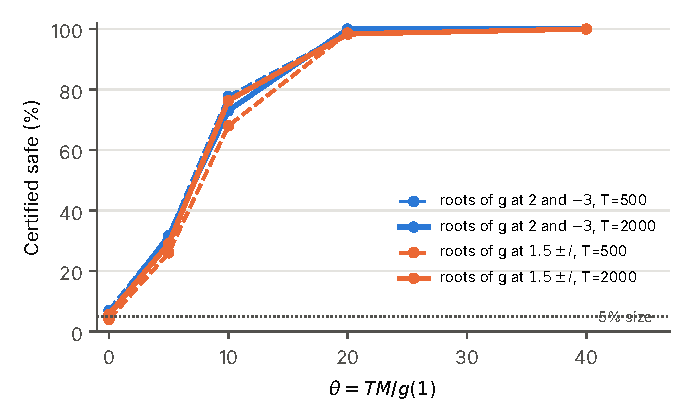
\includegraphics[width=0.72\textwidth]{fig_uniform_power.pdf}
\caption{Simulated success of the augmented Dickey--Fuller certificate at the 5\% level as a function of $\theta=TM/g(1)$, for two root structures of $g$ and two record lengths. The curves collapse onto one, as Theorem~\ref{thm:uniform} says: the margin matters only through $TM/g(1)$. 300 replications per point.}\label{fig:uniform}
\end{figure}

In simulation (Figure~\ref{fig:uniform}) the certification rate depended on the margin only through $TM/g(1)$: across two choices of $g$ and $T\in\{500,2000\}$ it was \UniformPowerZero--\UniformPowerZeroHi\% at $\theta=0$, \UniformPowerTenLo--\UniformPowerTenHi\% at $\theta=10$ and at least \UniformPowerForty\% at $\theta=40$.

\subsection{Contrarian agents and worst-case loss}\label{sec:signed}

\begin{proposition}[Contrarian agents]\label{prop:signed}
Allow signed weights, so that the merged measure is signed with total variation at most $B$.
\begin{enumerate}[label=(\roman*)]
\item Linear questions, including $\Phi$, cost at most a constant factor more than in the positive class: the modulus of continuity at most doubles.
\item The summed response no longer measures risk. The worst-case loss is $|I|\bar w\|h\|_1\ge|I|\bar w|S|$, and $\|h\|_1/|S|$ is unbounded on stable economies with a memory bound: one contrarian cohort with memory rate zero and $a+\kappa q=-q_0$, $q_0\in[0,1)$, has $h_t=\kappa(-q_0)^{t-1}$, $|S|=\kappa/(1+q_0)$ and $\|h\|_1=\kappa/(1-q_0)$.
\item The horizon-limited worst case $\bar w\|h\|_{1,H}$ is certified from reset experiments with no memory bound and no sign condition, at a cost of order $\sigma^2H^2\epsilon^{-2}$ instead of $\sigma^2H\epsilon^{-2}$ in the positive class.
\end{enumerate}
\end{proposition}

\begin{proof}
(ii) With memory rate zero, $k_0=q$ and $h_{t+1}=(a+\kappa q)h_t$ with $h_1=\kappa$; sum the geometric series. Parts (i) and (iii) are proved in \citet[Proposition~4.9.1]{niroula2026thesis}.
\end{proof}

With $\psi_j$ the coefficients of $1/f$, a shock sequence of $k$ innovation standard deviations moves the displacement by at most $k\sigma\Psi_H$ within $H$ periods, $\Psi_H=\sum_{j<H}|\psi_j|$, and some sequence attains it.

\begin{theorem}[Passive certificate of worst-case loss]\label{thm:absresp}
On a compact set of stationary finite-memory economies with signed kernels, the interval $\Psi_H(\hat\phi)\pm G_H(\chi^2_{L,1-\alpha}\lambda_{\max}(\hat\Sigma)/T)^{1/2}$, with $G_H$ a Lipschitz constant of $\Psi_H$ and $\hat\Sigma$ the estimated covariance of the least-squares coefficients, covers $\Psi_H$ with probability at least $1-\alpha+o(1)$ uniformly; its half-width is of order $T^{-1/2}$, and no interval does better than order $T^{-1/2}$. The summed response $1/M$ can understate $\Psi_\infty$ by an unbounded factor.
\end{theorem}

\begin{proof}
Uniform asymptotic normality of $\hat\phi$ on compact sets of stationary autoregressions \citep{mannwald1943,mikusheva2007}, the polynomial dependence of each $\psi_j$ on $\phi$, and $\big||u|-|v|\big|\le|u-v|$ give the upper bound. For the lower bound, $\Psi_H=\sum_{j<H}\rho^j$ in the memory-zero economies is strictly increasing with derivative at least one, and roots $\rho$ and $\rho+\delta T^{-1/2}$ have divergence bounded in $T$.
\end{proof}

In a simulated contrarian economy the interval covered $\Psi_H$ in \UniformCover\% of replications, and the summed response understated it by \UniformUnderstate\%. The margin is the right statistic for whether a market is stable, in either class; it is the right statistic for worst-case loss only in the positive class.

\section{Evidence}\label{sec:evidence}

\subsection{Data and design}

All tests use Binance USD-M perpetual futures from the exchange's public archive (\texttt{data.binance.vision}): one-minute klines with taker-buy volume, which give the last price and the signed taker notional of each minute, aggregated to five-minute marks. A day is valid if at least half of its five-minute returns are non-zero and its flow is not identically zero; a market is evaluable with at least 200 valid days. On each valid day the sufficient statistics of the two regressions in~\eqref{eq:reduced} are computed and pooled over days, and the margin is $\hat M=-\hat\beta-\hat\kappa\hat\Phi$, decided if its 95\% day-bootstrap interval (200 draws) excludes zero. The memories are identified if a two-exponential fit to the return kernel separates two rates with a bootstrap interval excluding zero and neither rate's interval touching a bound of the fit.

Each test's specification, the hashes of its code, its universe rule and its seed were pushed to a public repository in a commit of their own before any of its data were downloaded (Appendix~\ref{app:registry}). The code refuses to run if any hash differs or the specification is not committed, and a counter that the code increments on opening prevents a second run. Universes are drawn in a seeded random order from symbols that appear in no file of the repository, so every test uses markets never used before. Results are reported as they came out, and explanations found afterwards are labelled post hoc. Table~\ref{tab:registered} lists every registered primary hypothesis of the project and its result.

\begin{table}[p]\centering\footnotesize
\begin{threeparttable}
\caption{Every registered primary hypothesis and its result}\label{tab:registered}
\begin{tabular}{>{\raggedright\arraybackslash}p{0.06\textwidth}>{\raggedright\arraybackslash}p{0.52\textwidth}>{\raggedright\arraybackslash}p{0.32\textwidth}}
\toprule
Test & Primary hypothesis & Result\\
\midrule
E1 & 1. Certifying the summed response is at least 10 times more precise than separating memories & failed: \EonePone{} of \EoneSymbols{} symbols (\EoneNeed{} needed)\\
 & 2. Price-only memory intervals are at least 10 times wider than class-tagged ones & passed: \EonePtwo{} of \EoneSymbols{}\\
D1 & 1. Class-tagged interval width falls with slope in $[-0.75,-0.25]$ & failed: \DonePone{} of \DoneSymbols{} (\DoneNeed{} needed)\\
 & 2. The advantage of tagging grows with the sample & passed: \DonePtwo{} of \DoneSymbols{}\\
G1 & 1. Amplification-adjusted volatility limit beats a volatility limit in stress hours & failed: identical rules ($\theta=\GoneTheta$)\\
 & 2. The summed-response guard beats a volatility limit in stress hours & failed: tail-loss ratio \GoneGuardPct{} higher\\
V1 & 1. The depth-free statistic forecasts excursions in thin Kraken pairs & failed: $\Delta R^2=\VoneDeltaRtwo$ points\\
 & 2. It beats an order-splitting placebo & not tested\\
O1 & After scheduled US macro releases, small perpetuals overshoot & failed: $\bar A_{120}=\OoneAbar$ s, interval \OoneCI{}\\
C2 & 1. The margin is decided in at least 75\% of 30 new markets & failed: \CtwoDecided{} of \CtwoSymbols{} (\CtwoNeed{} needed)\\
 & 2. Decided but not identified outnumbers identified but not decided & passed: \CtwoB{} against \CtwoC{}\\
 & 3. At a matched horizon, class-tagged persistence is tighter than price-only memory & passed: \CtwoPthreeTighter{} of \CtwoPthreeSymbols{} (\CtwoPthreeNeed{} needed)\\
C3 & 1. With 430 days, the margin is decided in at least 75\% of new markets & passed: \CthreeDecided{} of \CthreeSymbols{} (\CthreeNeed{} needed)\\
 & 2. Decided but not identified outnumbers the reverse & passed: \CthreeB{} against \CthreeC{}\\
F1 & 1. The margin is decided in at least 75\% of new markets & passed: \FoneDecided{} of \FoneSymbols{} (\FoneNeed{} needed)\\
 & 2. Decided but not identified outnumbers the reverse & passed: \FoneB{} against \FoneC{}\\
 & 3. The 20-day margin forecasts the next day's largest adverse move & failed: $t=\FoneRiskT$, $p=\FoneRiskP$\\
S1 & 1. On stress days, markets with a lower prior margin are hit harder & failed: mean partial correlation \SoneRho{}\\
 & 2. A lower margin forecasts next-day realized variance & passed: $t=\SoneRvT$\\
 & 3. It does so beyond the Hawkes branching ratio & passed: $t=\SoneHawkesT$\\
 & 4. A lower margin forecasts next-day extreme moves & failed: $t=\SoneTailT$, Holm $p=\SoneTailPholm$\\
R1 & 1. Next-day adverse moves rise with the absolute response $\Psi_H$ & passed: elasticity \RoneElast{} (\RoneElastSE)\\
 & 2. $\Psi_H$ forecasts adverse moves, positive coefficient & failed: coefficient \RoneFcCoef{}\\
 & 3. It does so beyond the margin & failed: coefficient \RoneBeyondCoef{}\\
H1 & 1. Real accounts have distinct memories their records reveal & prospective; opens 10 December 2026\\
 & 2. Prices and anonymous flow do not reveal them & prospective; opens 10 December 2026\\
\bottomrule
\end{tabular}
\begin{tablenotes}\footnotesize\item Holm's correction across the primaries of each test (a fixed sequence for V1). E1, D1 and the first part of the project used other designs, reported in the companion thesis. Sources: the committed result files of each test, checked against their registered specification hashes by the project's verification script.\end{tablenotes}
\end{threeparttable}
\end{table}

\subsection{Certification without identification}

\begin{table}[ht]
\centering\small
\begin{threeparttable}
\caption{Registered tests of the dichotomy}\label{tab:tests}
\begin{tabular}{lccc}
\toprule
 & C2 & C3 & F1\\
\midrule
New markets drawn / evaluable & \CtwoSymbols{} / \CtwoSymbols{} & \CthreeDrawn{} / \CthreeSymbols{} & \FoneDrawn{} / \FoneSymbols{}\\
Days per market & 105 & 430 & 430\\
Margin decided (registered threshold) & \CtwoDecided{} (\CtwoNeed{}) & \CthreeDecided{} (\CthreeNeed{}) & \FoneDecided{} (\FoneNeed{})\\
\quad of which unsafe & 0 & 0 & 0\\
Memories identified & \CtwoIdentified{} & \CthreeIdentified{} & \FoneIdentified{}\\
Decided, not identified : identified, not decided & \CtwoB{} : \CtwoC{} & \CthreeB{} : \CthreeC{} & \FoneB{} : \FoneC{}\\
Same decision without the feedback term & \CtwoSameNoFb{} & \CthreeSameNoFb{} & \FoneSameNoFb{}\\
Feedback term negative (contrarian) & \CtwoFbNeg{} & \CthreeFbNeg{} & \FoneFbNeg{}\\
\bottomrule
\end{tabular}
\begin{tablenotes}\footnotesize\item C2 used 105 dates; C3 and F1 used 430 dates from January 2025 to September 2026 and C3's valid-day rule. Markets with fewer than 200 valid days were excluded under that rule.\end{tablenotes}
\end{threeparttable}
\end{table}

\begin{figure}[ht]\centering
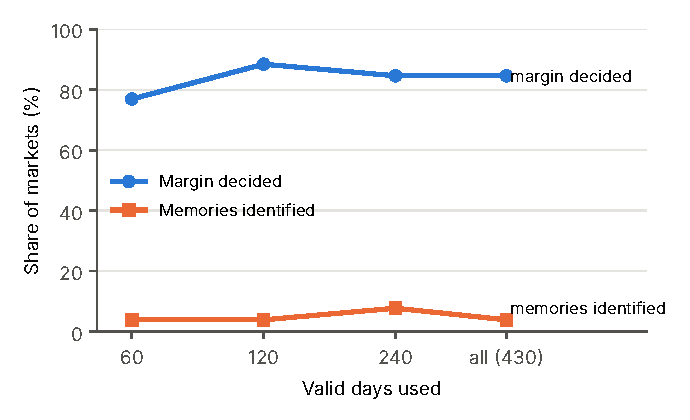
\includegraphics[width=0.72\textwidth]{fig_learning_curve.pdf}
\caption{Test F1, registered secondary: share of the \FoneSymbols{} evaluable new markets in which the margin was decided and in which the memories were identified, using the first 60, 120 and 240 valid days and all of them.}\label{fig:curve}
\end{figure}

Table~\ref{tab:tests} and Figure~\ref{fig:curve} give the result. With 105 days per market the margin was decided in \CtwoDecided{} of \CtwoSymbols{}, one short of the threshold; with 430 days, in \CthreeDecided{} of \CthreeSymbols{} and \FoneDecided{} of \FoneSymbols{}, and on the first 105 days of C3's markets in \CthreeFirst{}: the decision comes with the length of the record, as Theorem~\ref{thm:passive} predicts. Every decided margin was on the safe side, and the memories were identified in at most one market per test. Quarter by quarter, in an exploratory analysis of \PsixSQ{} symbol-quarters, the margin was decided in \PsixDecided{}, never on the unsafe side.

Two qualifications matter. The decision rests mainly on reversion: without the feedback term it was the same in most markets, so these data certify that the markets are far from the boundary without measuring the feedback precisely. And the prediction that the standardized margin grows like the square root of the record holds across markets but not market by market, because the margin drifts; the drift calibration above puts most of these markets between the two ends of the drift floor.

\subsection{Disclosure}

Binance publishes five-minute long/short positioning ratios for a top-trader class and for all accounts. In C2 a registered primary compared the width of the interval for the class persistence rate with that of the price-only slow memory from a kernel matched to the class horizon (eight hours). The class interval was narrower in \CtwoPthreeTighter{} of \CtwoPthreeSymbols{} markets, by a median factor of \CtwoRatio{} (smallest \CtwoMinRatio{}). A registered secondary qualifies what this measures: corrected for the downward bias of day-demeaned regressions, the median class persistence was \CtwoJackR{} per five minutes, and below one in only \CtwoJackBelow{} of \CtwoClassFits{} class fits. Positioning data restrict a persistence parameter that prices cannot bound; whether it reflects learning memory or slow turnover of positions, these data do not say. Test H1 below is designed to answer that with participant-level data.

\subsection{The certificate and risk}\label{sec:s1}

\paragraph{F1.} A third registered primary of F1 asked whether the margin estimated on the previous 20 valid days forecasts the next valid day's largest adverse move out of sample, beyond realized variance, in a pooled model with symbol fixed effects and Clark--West loss differentials averaged within dates. The coefficient had the predicted sign (\FoneRiskCoef{}), but the test failed ($t=\FoneRiskT$, $p=\FoneRiskP$). For next-day realized variance, a registered secondary, the same design gave $t=\FoneRvT$.

\paragraph{S1.} Test S1 was registered on 25 October 2026 on \SoneDrawn{} further markets and every day from January 2025 to September 2026 (\SoneSymbols{} evaluable). Two of its four primaries passed. A lower margin forecast higher next-day realized variance out of sample (coefficient \SoneRvCoef{}, Clark--West $t=\SoneRvT$, Holm-adjusted $p=\SoneRvP$, gain \SoneRvGain{} points of $R^2$ on \SoneDates{} test dates), and the forecast was unchanged when the branching ratio of a Hawkes model of trade arrivals, estimated by the INAR approximation of \citet{kirchner2016}, was added to both models ($t=\SoneHawkesT$); the branching ratio alone did not forecast variance ($t=\SoneNhatRvT$). Two failed. On the 20 worst market-wide days the prior margin did not rank which markets were hit hardest (mean partial rank correlation \SoneRho{}), and the forecast of next-day extreme moves fell short ($t=\SoneTailT$, Holm $p=\SoneTailPholm$). As a secondary, the branching ratio did rank stress-day damage, but with the sign opposite to the criticality reading: markets with a higher prior branching ratio had smaller adverse moves (mean partial correlation \SoneNhatStressRho{}).

\paragraph{R1.} Test R1, registered the same day on \RoneDrawn{} further markets (\RoneSymbols{} evaluable, none shared with S1), asked whether the estimated absolute response $\Psi_H$ of Theorem~\ref{thm:absresp}, with $H$ one hour, does what the margin did not. Within markets the next day's log adverse move rose with log $\Psi_H$, instrumented by its lag and controlling for shock size: elasticity \RoneElast{} (standard error \RoneElastSE{}), positive as predicted, about half the theory's value of one; for variance the elasticity was \RoneRv{} against two. Out of sample and beyond recent volatility, however, a larger $\Psi_H$ forecast a smaller adverse move (coefficient \RoneFcCoef{}), so the two registered forecasting primaries, which required a positive coefficient, failed. The data do not separate $\Psi_H$ from the summed response: at a one-hour horizon the estimated responses rarely change sign (median $\Psi_H/|S_H|=\RoneRatio$), the elasticity is the same in contrarian and momentum markets (\RoneContr{} and \RoneMom), and $S=\kappa/M$ itself has elasticity \RoneLogS{}.

\paragraph{Reading.} The certificate measures how close a market is to instability, and in these data it carries information about the coming day's turbulence that the standard measure of self-excitation does not. It does not tell where a crash will land, and the size of the estimated response, though it scales with losses, adds nothing in the predicted direction once recent volatility is known.

\subsection{Real agents}\label{sec:h1}

H1 is prospective and uses participant-level data. Hyperliquid, a perpetual-futures exchange whose order book runs on a public blockchain, publishes every trade with the buyer's and the seller's wallet address. H1 was registered before any of its data existed; a collector records every trade in 30 markets, ranked 11 to 40 by volume when collection started, and the analysis opens once at least 20 markets have 30 days of near-complete recording. For the ten largest accounts in each market it estimates each account's memory, the persistence of its position, and its response to the displacement, and asks whether two accounts have distinguishable memories in at least 75\% of markets, and whether prices and anonymous flow fail to separate memories where the accounts' own records succeed. It is the first test of the identification theory against real agents rather than proxies. Its limits were stated at registration: addresses are accounts, not firms or algorithms, and positions are reconstructed only from the start of collection.

\section{Robustness (exploratory)}\label{sec:robust}

The analyses in this section were chosen after the registered results were known and are not confirmatory. They use the committed data rows of S1 and R1.

\begin{table}[ht]
\centering\small
\begin{threeparttable}
\caption{Exploratory robustness of S1's variance forecast and R1's size elasticity}\label{tab:robust}
\setlength{\tabcolsep}{3pt}
\begin{tabular}{lrr@{\hspace{0.5em}}lrr}
\toprule
\multicolumn{3}{c}{S1: margin forecasts next-day variance} & \multicolumn{3}{c}{R1: elasticity of adverse move}\\
Variant & coef. & $t$ & Variant & elasticity & s.e.\\
\midrule
Registered & \RobSBaseC & \RobSBaseT & Registered & \RobRBaseE & \RobRBaseSE\\
Clustered by week & \RobSWeekC & \RobSWeekT & With volatility controls & \RobRVolE & \RobRVolSE\\
Clustered by market & \RobSSymC & \RobSSymT & 2025 only & \RobRYrAE & \RobRYrASE\\
Training share 50\% & \RobSTrFiftyC & \RobSTrFiftyT & 2026 only & \RobRYrBE & \RobRYrBSE\\
Training share 70\% & \RobSTrSeventyC & \RobSTrSeventyT & Impact $\hat\kappa$ alone & \RobRKappaE & \RobRKappaSE\\
Winsorized at 1/99\% & \RobSWinsC & \RobSWinsT & $\log S$, shock control & \RobRSShockE & \RobRSShockSE\\
2025 only & \RobSYrAC & \RobSYrAT & $\log S$, Pilot~7's control & \RobRSPsevenE & \RobRSPsevenSE\\
2026 only & \RobSYrBC & \RobSYrBT & & & \\
Without October 2025 & \RobSNoOctC & \RobSNoOctT & & & \\
High-volatility markets & \RobSHiVolC & \RobSHiVolT & & & \\
Low-volatility markets & \RobSLoVolC & \RobSLoVolT & & & \\
Leave one market out ($t$ range) & & \RobSLooMin--\RobSLooMax & Leave one market out (range) & \multicolumn{2}{r}{\RobRLooMin--\RobRLooMax}\\
\bottomrule
\end{tabular}
\begin{tablenotes}\footnotesize\item Left: S1's pooled out-of-sample forecast of next-day $\log(1+\mathrm{RV})$ from the winsorized 20-day margin, Clark--West $t$ with differentials averaged within the clustering unit (dates unless stated). Right: R1's 2SLS elasticity of next-day $\log(1+\mathrm{MAE})$, instrumented by the lagged-window estimate, standard errors clustered by date. Pilot~7's control multiplies the flow shock by the estimated impact.\end{tablenotes}
\end{threeparttable}
\end{table}

\begin{figure}[ht]\centering
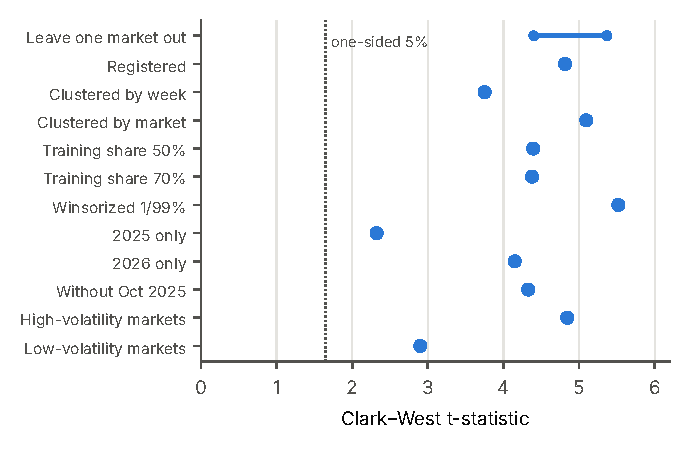
\includegraphics[width=0.72\textwidth]{fig_robustness.pdf}
\caption{Exploratory robustness of S1's registered variance forecast: Clark--West $t$-statistics under alternative clustering, training shares, winsorization, subperiods and subsamples, and the range when any one market is removed.}\label{fig:robust}
\end{figure}

Table~\ref{tab:robust} and Figure~\ref{fig:robust} give two different pictures. S1's variance forecast is stable: the $t$-statistic stays between \RobSYrAT{} and \RobSWinsT{} across clustering units, training shares, winsorization, calendar years, the exclusion of October 2025, volatility halves, and the removal of any single market. R1's elasticity is not. It was \RobRYrAE{} in 2025 and \RobRYrBE{} in 2026, it fell to \RobRVolE{} with recent volatility in the regression, and the estimated impact $\hat\kappa$ alone, the first tap of the response, had elasticity \RobRKappaE{}: the registered result mostly says that days of higher estimated impact are followed by larger moves. The same rows also settle the sign of Pilot~7: with the control Pilot~7 used, which multiplies the shock by the estimated impact, the elasticity of $S$ is \RobRSPsevenE{}; with the shock alone it is \RobRSShockE{}. The negative sign was a property of that specification, not of contrarian agents.

\section{Discussion}\label{sec:discussion}

\paragraph{For supervisors.} The results separate two questions that are often run together. Whether a market is stable can be certified from public data, at a cost set by its distance from instability, without identifying any agent; who is trading cannot be learned from market data at any comparable cost. Three practical implications follow. First, a supervisor who cares about stability should estimate the margin, with the pooled estimator and a window matched to the drift of the market, and treat identification as a separate task with its own justification. Second, disclosure has a precise role in certification: it must bound the memory of the largest participants, because without such a bound no passive certificate exists (Theorem~\ref{thm:hidden}). Requirements that reveal identities without bounding memory do not help stability supervision. Third, the margin should not be read as a crash indicator. In our data it forecast turbulence and did not rank damage on the worst days.

\paragraph{For research.} The tests used one venue and one asset class, and every certified market was far from the boundary. Two open questions matter most. The first is whether the margin falls before genuine near-boundary episodes; this needs events that the present sample does not contain, or a market designed to be near the boundary. The second is whether real agents' memories are distinct and invisible to prices, which H1 answers with participant-level data. On the theory side, the uniform result for geometric memory and for the pooled estimator's nuisance parameters remain open, as does the gap between the moving-average displacement and the distance from fundamental value.

\paragraph{Limits.} The model is linear and its agents respond to one state. Real algorithms use many signals, change their parameters, and trade across venues. The companion thesis shows that the stability bound survives nonlinear rules and time-varying agents given a bound on their total sensitivity, but our estimators and tests use the linear form. The exogeneity of contemporaneous flow to price noise is an assumption of the pooled estimator that five-minute data can violate.

\section{Conclusion}

A supervisor with public data can learn how close a market is to feedback instability, at a cost set by that distance, without learning who trades in it; learning who trades costs polynomially more and does not get cheaper by watching. The one input prices cannot supply is a bound on how slowly the largest participants trade. In crypto perpetual futures the certificate behaves as the theory says for stability and forecasts the coming day's turbulence beyond the standard measure of self-excitation; it does not forecast crashes. Every one of these statements rests on tests whose design was public before their data were.

\paragraph{Acknowledgements and disclosure.} Code, proofs and text were drafted with the assistance of Claude (Anthropic), an AI system; the authors checked and are responsible for all content. Arithmetic steps of the proofs are checked in Lean~4 with Mathlib (modules \texttt{ThesisPassiveMulti}, \texttt{ThesisHidden}, \texttt{ThesisPooled} and companions). Specifications, code, results and the checks that regenerate every number in this paper are in the public repository \url{https://github.com/Pratikn03/Fianince}.

\appendix
\section{Proofs}\label{app:proofs}

\paragraph{Theorem~\ref{thm:passive}.} (i) Both economies are $x_{t+1}=\rho_jx_t+e_{t+1}$ with $e_{t+1}\sim N(0,\kappa^2s^2)$, $\rho_0=1-\mu$, $\rho_1=1+\mu$. The divergence is $\tfrac12(2\mu)^2\sum_{t<T}v_t$ with $v_0=0$, $v_{t+1}=\rho_0^2v_t+1$, so $v_t\le1/(1-\rho_0^2)\le1/\mu$ and the divergence is at most $2T\mu$. By Pinsker's inequality the total variation distance is at most $(T\mu)^{1/2}$, while a procedure with error at most $\alpha$ under both separates them with total variation at least $1-2\alpha$. (ii) For fixed $|\rho|<1$, $\sqrt T(\hat\rho-\rho)\to N(0,1-\rho^2)$ \citep{mannwald1943} and $1-\rho^2=M(2-M)$. Along $\rho_T=1-M_T$ with $M_T\to0$, $TM_T\to\infty$, \citet{phillips2007} give $(T/2M_T)^{1/2}(\hat\rho-\rho_T)\to N(0,1)$; since $\hat M/M_T\to1$ in probability, the studentized interval has asymptotic coverage $1-\alpha$ and excludes zero once $M>z_{1-\alpha/2}(2M/T)^{1/2}$.

\paragraph{Theorem~\ref{thm:multi}.} (i) $g$ is real on $[0,1]$, equals one at zero and has no zero there, so $g(1)>0$. Both economies have finite memory, since any real $\phi$ arises from $k_i=\phi_i/\kappa$, $i\ge1$, and $a=\phi_0-\kappa k_0$. The divergence is $\sum_{t<T}\E_+[((f_+-f_-)(\mathcal L)x_{t+1})^2]/(2\sigma^2)$, and $(f_+-f_-)(z)=(\rho_--\rho_+)zg(z)$, so it equals $(2\mu/g(1))^2\sum_{t<T}\E_+y_t^2/(2\sigma^2)$ with $y_t=g(\mathcal L)x_t$. Under $f_+$, $y_{t+1}=\rho_+y_t+e_{t+1}$ from $y_0=0$, so $\E_+y_t^2\le\sigma^2/(1-\rho_+^2)\le\sigma^2g(1)/\mu$, and the divergence is at most $2T\mu/g(1)$. Pinsker's inequality finishes.

(ii) The regression is an invertible reparametrization of the stationary autoregression of $x_{t+1}$ on $x_t,\dots,x_{t-p}$, so by \citet{mannwald1943} the coefficients are asymptotically normal with covariance $\sigma^2\Gamma^{-1}$, and the entry for $x_t$ is $1/\tau^2$, with $\tau^2$ the residual variance of $x_t$ after projection on the lagged differences. Each such residual is $h(\mathcal L)x_t$ with $h$ a polynomial of degree at most $p$ and $h(1)=1$. With $\delta=1-\rho$, $G=\max_{|z|=1}|g|$ and $|1-\rho e^{-i\lambda}|^2\le\delta^2+\lambda^2$,
\[
\tau^2\ge\frac{\sigma^2}{2\pi G^2}\min_h\int_{-\pi}^{\pi}\frac{|h(e^{-i\lambda})|^2}{\delta^2+\lambda^2}\,d\lambda .
\]
Let $H(\lambda)=h(e^{-i\lambda})$ and $I$ the integral. Since $\delta^2+\lambda^2\le1+\pi^2$, $\int|H|^2\le(1+\pi^2)I$; by Cauchy--Schwarz $\max|H|^2\le(p+1)\int|H|^2/(2\pi)$, and by Bernstein's inequality $\max|H'|\le p\max|H|$, so $\max|H'|\le pB\sqrt I$ with $B^2=(p+1)(1+\pi^2)/(2\pi)$. With $r=\min(\pi,1/(2pB\sqrt I))$, $|H|\ge1/2$ on $|\lambda|\le r$, so $I\ge\arctan(r/\delta)/(2\delta)$. If $r\ge\delta$ this is at least $\pi/(8\delta)$; otherwise $r=1/(2pB\sqrt I)<\delta$ and $I>1/(4p^2B^2\delta^2)$. Hence $I\ge c/\delta$ with $c=1/(4p^2B^2)$, $\tau^2\ge\sigma^2c/(2\pi G^2\delta)$, and with $\delta=M/g(1)$, $V=\sigma^2/\tau^2\le4p^2(p+1)(1+\pi^2)G^2M/g(1)$. Finally $g(z)=\prod_j(1-z/r_j)$ with $|r_j|\ge1+\gamma$ gives $G\le2^p$ and $g(1)\ge(\gamma/(1+\gamma))^p$.

\paragraph{Theorem~\ref{thm:pooled}.} (i) With one cohort of memory rate zero, $f_{t+1}=qx_t+w_{t+1}$ and $x_{t+1}=ax_t+\kappa f_{t+1}+\varepsilon_{t+1}$. The conditional density of $(f_{t+1},x_{t+1})$ factorizes into the flow equation and the price equation given the flow, and the second is the same under both economies, so the divergence is $\sum_{t<T}\E_+(q_+-q_-)^2x_t^2/(2s_w^2)$ with $|q_+-q_-|=2\mu/\kappa$. Under the safe economy $x_{t+1}=(1-\mu)x_t+\kappa w_{t+1}+\varepsilon_{t+1}$, so $\E_+x_t^2\le\sigma^2/\mu$ with $\sigma^2=\kappa^2s_w^2+s_\varepsilon^2$, and the divergence is at most $2T\mu(1+R)$. (ii) Write $\hat M-M=-(\hat\beta+\hat\kappa\Phi+M)-\hat\kappa(\hat\Phi-\Phi)$. Both regressions are equations of a stationary Gaussian vector autoregression whose regressors are uncorrelated with their errors, so the estimators are jointly asymptotically normal and $\hat\kappa\to\kappa$. In the flow equation, reparametrized with $x_t$ and $p$ lagged differences, the coefficient on $x_t$ is $\Phi$, so $\hat\Phi$ has asymptotic variance $s_w^2/\tau^2$ with $\tau^2$ as above, and $\kappa^2s_w^2/\tau^2\le2\pi G^2\delta/c$. In the price equation, with $\tilde w_{t+1}=f_{t+1}-\Phi x_t$, the regression on $(f_{t+1},x_t)$ is a reparametrization of that on $(\tilde w_{t+1},x_t)$ in which the coefficient on $x_t$ is $-M$; since $\tilde w_{t+1}$ lies in the span of $w_{t+1}$ and the lagged differences and $w_{t+1}$ is independent of them and of $x_t$, the residual variance of $x_t$ after projection on $\tilde w_{t+1}$ is at least $\tau^2$, and $\hat\beta+\hat\kappa\Phi+M$ has asymptotic variance at most $s_\varepsilon^2/\tau^2\le2\pi G^2\delta/c$. By $(u+v)^2\le2u^2+2v^2$, $V_{\rm pool}\le8\pi G^2\delta/c=4\cdot2\pi G^2M/(c\,g(1))\le4C_{p,\gamma}M$.

\paragraph{Theorems~\ref{thm:hidden}, \ref{thm:uniform} and~\ref{thm:absresp}.} The proofs in the text are complete up to the cited limit theory. For Theorem~\ref{thm:hidden}, under $\mathcal E_0$, $\E_0x_s^2\le\sigma^2/(1-(1-c)^2)\le\sigma^2/c$, and $\sum_{t<T}(t+1)^2\le T^3$; Pinsker's inequality gives $\mathrm{TV}\le(\mathrm{KL}/2)^{1/2}$, which tends to zero as $r\uparrow1$ for fixed $T$, and a procedure with error at most $\alpha$ under both economies needs $2(1-2\alpha)^2\le\mathrm{KL}$. The arithmetic steps of all five proofs are checked in Lean~4 (Appendix~\ref{app:registry}).

\section{Registration record}\label{app:registry}

\begin{table}[ht]
\centering\footnotesize
\begin{threeparttable}
\caption{Registration of the tests reported in Section~\ref{sec:evidence}}\label{tab:registry}
\begin{tabular}{llll}
\toprule
Test & Specification SHA-256 (first 12) & Registration commit & Opened\\
\midrule
C2 & \texttt{aca63504f2ed} & \texttt{4a20531} & 2026-10-24\\
C3 & \texttt{9a4548277fb1} & \texttt{f8916b6} & 2026-10-25\\
F1 & \texttt{f6320484b223} & \texttt{b2e78b6} & 2026-10-25\\
S1 & \texttt{5dc805bb820c} & \texttt{b43f5b0} & 2026-10-25\\
R1 & \texttt{c597bbd7b1a4} & \texttt{68bbb75} & 2026-10-25\\
H1 & \texttt{833b1993b2f2} & \texttt{a7a00df} & opens from 2026-12-10\\
\bottomrule
\end{tabular}
\begin{tablenotes}\footnotesize\item Specifications are in \texttt{thesis/checks/prereg/} of the repository, with their hashes and counters. Each test's code verifies the specification hash and the hashes of every pipeline file before running and increments the counter on opening. F1's addendum A1, which restricted the universe filter to ASCII symbol names after a symbol written in Chinese characters stopped the first run before any data were downloaded, was registered in a commit of its own before the run resumed.\end{tablenotes}
\end{threeparttable}
\end{table}

\begin{thebibliography}{99}
\bibitem[Bacry et~al.(2015)]{bacry2015} Bacry, E., Mastromatteo, I. and Muzy, J.-F. (2015). Hawkes processes in finance. \emph{Market Microstructure and Liquidity} 1(1), 1550005.
\bibitem[Blough(1992)]{blough1992} Blough, S.~R. (1992). The relationship between power and level for generic unit root tests in finite samples. \emph{Journal of Applied Econometrics} 7(3), 295--308.
\bibitem[Bouchaud et~al.(2004)]{bouchaud2004} Bouchaud, J.-P., Gefen, Y., Potters, M. and Wyart, M. (2004). Fluctuations and response in financial markets: The subtle nature of `random' price changes. \emph{Quantitative Finance} 4(2), 176--190.
\bibitem[Brunnermeier and Pedersen(2009)]{brunnermeier2009} Brunnermeier, M.~K. and Pedersen, L.~H. (2009). Market liquidity and funding liquidity. \emph{Review of Financial Studies} 22(6), 2201--2238.
\bibitem[Budish et~al.(2015)]{budish2015} Budish, E., Cramton, P. and Shim, J. (2015). The high-frequency trading arms race: Frequent batch auctions as a market design response. \emph{Quarterly Journal of Economics} 130(4), 1547--1621.
\bibitem[Chan and Wei(1987)]{chanwei1987} Chan, N.~H. and Wei, C.~Z. (1987). Asymptotic inference for nearly nonstationary AR(1) processes. \emph{Annals of Statistics} 15(3), 1050--1063.
\bibitem[Dickey and Fuller(1979)]{dickeyfuller1979} Dickey, D.~A. and Fuller, W.~A. (1979). Distribution of the estimators for autoregressive time series with a unit root. \emph{Journal of the American Statistical Association} 74(366), 427--431.
\bibitem[Donoho(1992)]{donoho1992super} Donoho, D.~L. (1992). Superresolution via sparsity constraints. \emph{SIAM Journal on Mathematical Analysis} 23(5), 1309--1331.
\bibitem[Donoho(1994)]{donoho1994} Donoho, D.~L. (1994). Statistical estimation and optimal recovery. \emph{Annals of Statistics} 22(1), 238--270.
\bibitem[Elliott et~al.(1996)]{ers1996} Elliott, G., Rothenberg, T.~J. and Stock, J.~H. (1996). Efficient tests for an autoregressive unit root. \emph{Econometrica} 64(4), 813--836.
\bibitem[Faust(1996)]{faust1996} Faust, J. (1996). Near observational equivalence and theoretical size problems with unit root tests. \emph{Econometric Theory} 12(4), 724--731.
\bibitem[Filimonov and Sornette(2012)]{filimonov2012} Filimonov, V. and Sornette, D. (2012). Quantifying reflexivity in financial markets: Toward a prediction of flash crashes. \emph{Physical Review E} 85(5), 056108.
\bibitem[Hardiman et~al.(2013)]{hardiman2013} Hardiman, S.~J., Bercot, N. and Bouchaud, J.-P. (2013). Critical reflexivity in financial markets: A Hawkes process analysis. \emph{European Physical Journal B} 86, 442.
\bibitem[Harvey(2017)]{harvey2017} Harvey, C.~R. (2017). Presidential address: The scientific outlook in financial economics. \emph{Journal of Finance} 72(4), 1399--1440.
\bibitem[Harvey et~al.(2016)]{harvey2016} Harvey, C.~R., Liu, Y. and Zhu, H. (2016). \ldots and the cross-section of expected returns. \emph{Review of Financial Studies} 29(1), 5--68.
\bibitem[Hasbrouck(1991)]{hasbrouck1991} Hasbrouck, J. (1991). Measuring the information content of stock trades. \emph{Journal of Finance} 46(1), 179--207.
\bibitem[Heinrich and Kahn(2018)]{heinrich2018} Heinrich, P. and Kahn, J. (2018). Strong identifiability and optimal minimax rates for finite mixture estimation. \emph{Annals of Statistics} 46(6A), 2844--2870.
\bibitem[Ibragimov and Has'minskii(1984)]{ibragimov1984} Ibragimov, I.~A. and Has'minskii, R.~Z. (1984). On the nonparametric estimation of a value of a linear functional in Gaussian white noise. \emph{Theory of Probability and Its Applications} 29(1), 18--32.
\bibitem[Kirchner(2016)]{kirchner2016} Kirchner, M. (2016). Hawkes and INAR($\infty$) processes. \emph{Stochastic Processes and their Applications} 126(8), 2494--2525.
\bibitem[Kirilenko and Lo(2013)]{kirilenko2013} Kirilenko, A.~A. and Lo, A.~W. (2013). Moore's law versus Murphy's law: Algorithmic trading and its discontents. \emph{Journal of Economic Perspectives} 27(2), 51--72.
\bibitem[Kirilenko et~al.(2017)]{kirilenko2017} Kirilenko, A., Kyle, A.~S., Samadi, M. and Tuzun, T. (2017). The Flash Crash: High-frequency trading in an electronic market. \emph{Journal of Finance} 72(3), 967--998.
\bibitem[Kyle(1985)]{kyle1985} Kyle, A.~S. (1985). Continuous auctions and insider trading. \emph{Econometrica} 53(6), 1315--1335.
\bibitem[Mann and Wald(1943)]{mannwald1943} Mann, H.~B. and Wald, A. (1943). On the statistical treatment of linear stochastic difference equations. \emph{Econometrica} 11(3/4), 173--220.
\bibitem[Mikusheva(2007)]{mikusheva2007} Mikusheva, A. (2007). Uniform inference in autoregressive models. \emph{Econometrica} 75(5), 1411--1452.
\bibitem[Mikusheva(2012)]{mikusheva2012} Mikusheva, A. (2012). One-dimensional inference in autoregressive models with the potential presence of a unit root. \emph{Econometrica} 80(1), 173--212.
\bibitem[Niroula and Niroula(2026a)]{niroula2026a} Niroula, P. and Niroula, P. (2026a). Auditable memory and financial identification limits in electronic limit order books. Working paper.
\bibitem[Niroula(2026b)]{niroula2026thesis} Niroula, P. (2026b). From human markets to machine markets. Certify, don't identify: safety and identification in markets with adaptive trading agents. Thesis draft, Minnesota State University, Mankato.
\bibitem[Phillips(1987)]{phillips1987} Phillips, P.~C.~B. (1987). Towards a unified asymptotic theory for autoregression. \emph{Biometrika} 74(3), 535--547.
\bibitem[Phillips and Magdalinos(2007)]{phillips2007} Phillips, P.~C.~B. and Magdalinos, T. (2007). Limit theory for moderate deviations from a unit root. \emph{Journal of Econometrics} 136(1), 115--130.
\bibitem[P\"otscher(2002)]{potscher2002} P\"otscher, B.~M. (2002). Lower risk bounds and properties of confidence sets for ill-posed estimation problems with applications to spectral density and persistence estimation, unit roots, and estimation of long memory parameters. \emph{Econometrica} 70(3), 1035--1065.
\bibitem[Said and Dickey(1984)]{saiddickey1984} Said, S.~E. and Dickey, D.~A. (1984). Testing for unit roots in autoregressive-moving average models of unknown order. \emph{Biometrika} 71(3), 599--607.
\bibitem[Wu and Yang(2020)]{wu2020} Wu, Y. and Yang, P. (2020). Optimal estimation of Gaussian mixtures via denoised method of moments. \emph{Annals of Statistics} 48(4), 1981--2007.
\end{thebibliography}



% BEGIN ECONOMIC REVIEW 20261029
\section*{Development revision and validation status: 29 October 2026}
This is a working draft for author and specialist review. The revision corrects
hidden-state drift accounting, distinguishes cumulative displacement from peak
mark-to-market loss, and restricts claims to their stated model and observation
contracts. It does not declare every theorem independently verified or every
research objective complete.

\paragraph{Returned execution record.} The author returned a completed full-mode
notebook archive using source commit \texttt{19805d7e}, seed 20261029,
Python 3.13.18 and NumPy 2.1.3. All 10 exported-file hashes and the four analytical
source modules were checked. The run completed E1, E2, E3, E4 and E6; its log
reports 18 targeted tests passing. This is an execution reproduction of the same
seeded code, not independent scientific validation. No real-market CSV was
provided, and the GPU, known-source-feedback and prospective studies were not run.

\paragraph{What the checks establish.} E1 cross-checks the corrected drift identity
against a resolvent and exercises a sufficient invariant-box guard. E2 demonstrates
filter-induced persistence under martingale nulls. E3 compares known alternatives
with equal aggregate risk; it is an illustrative witness, not a uniform rate
theorem. E4 matches baseline capacity on training episodes and reports test
capacity differences; the guard and volatility control both have zero observed
budget breaches in the three bounded-shock synthetic regimes. This does not
establish universal guard superiority or economic welfare.

\paragraph{Coverage and the observation contract.} E6 uses 1,000 replications,
32 reset responses and 512 taps. The nominal 95\% interval assumes independent
Gaussian tap errors and a valid memory envelope. The intervals in the table
measure Monte Carlo uncertainty about coverage, not financial risk.
\begin{center}\small
\begin{tabular}{lrrc}
\toprule
Setting & Coverage & MC 95\% interval & Contract holds\\
\midrule
Independent Gaussian & 94.6\% & [93.0, 95.8] & yes\\
Correlated tap errors & 48.3\% & [45.2, 51.4] & no\\
Heavy-tailed readings & 95.1\% & [93.6, 96.3] & no\\
Biased readings & 25.6\% & [23.0, 28.4] & no\\
Unseen slow memory & 0.0\% & [0.0, 0.4] & no\\
\bottomrule
\end{tabular}
\end{center}
Failures under correlated errors, biased readings and a false memory floor expose
the contract's limits. The heavy-tail outcome in this configuration is not a
general robustness result. All outcomes, including negative ones, are retained.

\paragraph{Remaining obligations.} Independent review of the load-bearing
identification and certification proofs, continuous numerical extrema, economic
primitives, the public-observation bridge and policy counterfactuals remains
necessary. The current two-paper name-map audit finds 54 of 57 formal environments
with existing declaration mappings, three unmapped statements and seven revised
statements requiring semantic review. A label mapping is not a new Lean proof.
The experiment design and full results are retained under
\texttt{studies/economic\_review\_20261029/}.

% END ECONOMIC REVIEW 20261029

% BEGIN INFORMATION DECISION REVISION 20261029
\section*{Economic interpretation and returned decision experiment}

\subsection*{What this revision adds}
The information question is distinct from choosing a preferred amount of risk.
For a specified financial decision, the relevant issue is which observations
support an exposure constraint, what remains unidentified, and whether obtaining
additional information changes the attainable decision after costs. This does
not introduce portfolio choice or control without full identification as new
ideas. The general identification-versus-decision-value result still requires
independent proof and a comparison with the closest existing results.

\subsection*{Time conventions and the institution}
The new application is a price-taking, unlevered own-account investor, not a
venue-wide supervisor. It begins with cash, buys once, holds a fixed position
for 60 one-minute model periods, and closes fully. Round-trip linear and
quadratic charges enter cash and wealth. The account cannot change the market's
feedback, and the experiment does not measure customer liquidity or welfare.
This is separate from the paper's dealer/venue admission contracts.

\begin{center}\small
\begin{tabular}{p{0.26\textwidth}p{0.65\textwidth}}
\toprule
Quantity & Interpretation\\
\midrule
Sampling interval & One minute in the new synthetic account; other historical studies retain their stated sampling clocks.\\
Historical lookback & Often six hours in the existing forecasting studies; not a holding period.\\
Forecast horizon & Often the next hour's adverse excursion; not an executed round-trip trade.\\
New holding period & Exactly 60 model minutes, with explicit entry and exit charges.\\
Other theory horizons & The existing finite-horizon theorems retain their declared $H$; no universal holding period is imposed.\\
\bottomrule
\end{tabular}
\end{center}

\subsection*{Information and decision design}
The new comparison uses controlled independent reset observations of 12 impulse
taps, a known plant and reading variance, and a declared finite candidate class.
It does not treat public market trading as a reset experiment. Common training
and validation paths supply 768 and 384 additional reset episodes per repetition;
512 further paths evaluate the selected actions. These are in addition to the
reported tap-reading budget, not evidence of learning from 32 observations in
total. Verified disclosure restricts
the minimum-memory rate to an audited band. The oracle knows the true response,
not future shocks. All certificate arms use the same training objective.

The account selects a position by empirical expected logarithmic terminal
wealth, subject to its information-supported exposure restriction. This is a
finite-horizon application of logarithmic utility, not a newly proved Kelly
growth-optimality theorem. Equal response bounds alone do not imply equal
expected returns or identical utility-optimal portfolios.

The new account has initial wealth of 1,000 dollars and an initial price of
100 dollars; its position grid runs from zero to 9.9 units. Its round-trip
dollar charge is $c(I)=0.002I+0.0002I^2$. For bounded external flow, the
constraint adds this charge to position times the largest admissible absolute
price response over the holding horizon. The resulting bound concerns loss
from initial wealth at each date. It is not peak-to-trough drawdown, protection
against arbitrary unbounded shocks, or a rolling deployment guarantee.

\subsection*{Returned execution and proof scope}
The returned full-mode archive uses seed 20261029. All 35 manifest entries and
eight core source files were checked. The run contains 20 independent
repetitions per regime, not 16,800 independent experiments: the 16,800 policy
rows reuse tapes across policies, budgets and observation counts. Twelve
targeted checks passed. Eight conditional decision-logic lemmas compiled with
Lean 4.19.0 and their axiom printouts report no axioms. This is a seeded
execution reproduction. It neither completes the older manuscript's Lean
coverage nor formalizes the Gaussian confidence argument, market dynamics,
general minimax separation, portfolio optimality or welfare.

The displayed slice uses 32 reset episodes and a one-dollar loss budget from
initial wealth of 1,000 dollars. It is an illustrative presentation of an
exploratory grid, not a primary selected before the results were seen. All
regimes, budgets, policies and negative outcomes remain in the result archive.
The inputs and complete outputs are retained with the verification record in
the new information-decision study directory.

\subsection*{Aggregate information and unresolved cohorts: returned simulation}
\begin{center}\small
\begin{tabular}{lrrr}
\toprule
Regime & Unique candidate (\%) & Certified units & Oracle units\\
\midrule
No feedback & 0.0 & 9.405 & 9.900\\
Moderate feedback & 5.0 & 5.000 & 5.000\\
Near boundary & 0.0 & 1.200 & 1.200\\
\bottomrule
\end{tabular}
\end{center}
Here ``unique'' means one remaining candidate in the declared finite class,
not identification of arbitrary real-world algorithms. In the moderate and
near-boundary configurations, the aggregate certificate reaches the oracle's
grid capacity in this slice even though the candidate decomposition is usually
unresolved. This is an illustrative decision comparison; it does not prove a
uniform rate separation for continuous classes.

\subsection*{Disclosure cost and the negative result}
\begin{center}\small
\begin{tabular}{lrrr}
\toprule
Paid minus aggregate & Mean (bp) & Lower (bp) & Upper (bp)\\
\midrule
No feedback & -0.100 & -0.100 & -0.100\\
Moderate feedback & -0.126 & -0.126 & -0.125\\
Near boundary & -0.100 & -0.100 & -0.100\\
\bottomrule
\end{tabular}
\end{center}
The intervals are exploratory percentile bootstraps over repetition-level
paired means, not simultaneous intervals across the grid. In this slice the
unpaid disclosure does not expand capacity, while the assumed one-cent charge
reduces net log wealth. This run therefore does not establish a positive net
economic value of disclosure. The price is hypothetical, not a calibrated
reporting cost. Stronger disclosure need not be worth purchasing when aggregate
information already supports the relevant decision.

\subsection*{Assumption failures and calibration diagnostics}
The table reports finite-sample frequencies for all seven regimes, combining
the three reading budgets. Each band outcome is counted once per repetition
and reading budget (60 outcomes per regime); repeating the same outcome across
four financial loss budgets would not create further observations. The three
reading budgets within a repetition are not an independent replication.
\begin{center}\small
\begin{tabular}{lcrr}
\toprule
Regime & Contract valid & Tap-band hit (\%) & Empty set (\%)\\
\midrule
No feedback & Yes & 96.7 & 3.3\\
Moderate feedback & Yes & 93.3 & 5.0\\
Near boundary & Yes & 96.7 & 3.3\\
Hidden slow memory & No & 98.3 & 11.7\\
Correlated readings & No & 98.3 & 1.7\\
Biased readings & No & 0.0 & 100.0\\
Behaviour change & No & 95.0 & 5.0\\
\bottomrule
\end{tabular}
\end{center}
The nominal one-decision band coverage is 95 percent under the valid contract;
these small, dependent-budget frequencies are diagnostics, not a new coverage
theorem. A tap-band hit concerns the observed response, not membership in the
finite candidate class or stability of future behaviour. In particular, hidden
slow memory falls outside the declared class even when its first 12 taps fit
the bands. Under behaviour change the readings describe the old response.
Biased readings empty the set throughout this run and force the certificate
policy to abstain. Correlated readings use an unverified standard-error model.
None of these four regimes retains the stated guarantee; a high observed band
hit or zero observed financial breaches does not make an invalid contract valid.

\subsection*{Pending evidence: deliberately empty result cells}
The following numerical cells remain empty. The returned archive contained no
market CSV, dynamic-inventory experiment, institution-level intervention or
external replication. The general theorem and independent novelty review also
remain open; a table placeholder is not a theorem statement or a proof.

\begin{center}\small
\begin{tabular}{p{0.62\textwidth}cc}
\toprule
Pending study & Estimate & Uncertainty\\
\midrule
Untouched market-data test beyond order-flow imbalance and depth & & \\[1.8ex]
Full changing-inventory, execution and funding comparison & & \\[1.8ex]
Dealer/venue intervention with endogenous market response & & \\[1.8ex]
Net value under empirically calibrated disclosure costs & & \\[1.8ex]
Independent implementation and replication & & \\[1.8ex]
\bottomrule
\end{tabular}
\end{center}
\noindent Further data cannot by themselves prove a general identification or
decision-value theorem. Its exact statement, proof and literature priority
require separate review. No publication rating follows from the returned run.

% END INFORMATION DECISION REVISION 20261029

% BEGIN FINITE HORIZON COST 20261029
\section*{Finite-horizon information, cohort ambiguity, and net inventory-service value}

\paragraph{Status and contribution boundary.}
This appendix supplies a restricted analytic separation and its financial
consequence. The proof below is written in full; exact rational and numerical
checks accompany it. It has not received independent proof review and is not
a Lean formalization. Its priority is unconfirmed. Control without unique
identification, task-directed exploration, Gaussian functional estimation,
moment matching, and the value of information are established ideas
\citep{fhc:waarde,fhc:wagenmaker,fhc:donoho,fhc:heinrich,fhc:blackwell}.
The candidate extension is their explicit combination for a finite-horizon
inventory commitment, with a hard stress budget and the information bill
deducted from both capital and profit. It does not close the broader open
theorem of the preceding drafts.

\subsection*{The observation contract and the financial institution}
Fix $H\ge4$, $0\le a<1$, $\kappa>0$ and
$0\le Q\le\overline Q<(1-a)/\kappa$. There are arbitrarily many finite
cohorts, with $q_i\ge0$, $\sum_iq_i=Q$, and $0<\eta_i\le1$:
\[
 x_{t+1}=a x_t+\kappa\bigl(\sum_iq_i y_{i,t}+u_t\bigr),\qquad
 y_{i,t+1}=(1-\eta_i)y_{i,t}+\eta_i x_{t+1}.
\]
Initial states are reset to zero. Let $h_0,\ldots,h_{H-1}$ be the price
response to a unit impulse, with $h_0=\kappa$, and put
$G=\sum_{t<H}h_t$. Positivity implies $h_t\ge0$.
No positive lower bound on $\eta_i$ is imposed.

The observer purchases $N$ independent reset experiments, each lasting $H$
model periods and returning all $H$ taps with independent Gaussian errors of
known variance $\sigma^2$. Thus the tap means are
$\overline h_t=h_t+\sigma Z_t/\sqrt N$, with independent standard normal
$Z_t$. The same observations are available for identifying the cohorts and
for choosing the financial position. One experiment is not one scalar reading:
it returns $H$ readings and costs $c_H$, including the declared operating and
time charges. Total information cost is $F=Nc_H$. This observation contract
is not an ordinary exchange tape; longer horizons cost both time and readings.
Plant parameters, the feedback cap, reset, and stationarity are assumptions.
Measurements are acquired ahead of a common future service-start deadline.
Cash can earn the common reference rate during acquisition; the model does
not include earlier service opportunities. The stated measurement price is
exogenous, not a calibrated self-impact cost for actual market probes.

The institution is a price-taking, unlevered inventory-warehousing desk.
It buys $I\ge0$ units at $P_0$, holds them for $H$ periods, and closes.
It earns a prequoted service fee $pI$ \emph{after} settlement. Round-trip
execution and carry costs are $bI+dI^2$, where $b\ge0$ and $d>0$.
For example, $b=b_{\rm trade}+P_0 r_f H/(365\cdot24\cdot60)$ for
one-minute model periods. The service premium is unavailable as collateral
until after settlement. Both trading costs and $F$ must be prefunded.
Initial cash is $W$, the stressed-settlement loss budget is $B$, and
$|u_t|\le\overline u$, with $\overline u>0$. Assume
$P_0>\overline u\,\overline G$, so the asset price remains positive.
This desk does not alter market feedback, depth, or another participant's
behaviour. The service fee is exogenous, not an equilibrium price.

For the expected-profit objective, future shocks have conditional mean zero
given the observations. Consequently the conditional expected trading price
change is zero. The financial objective, including every declared charge, is
\[
 V(I,F)=g(I)-F,\qquad g(I)=(p-b)I-dI^2.
\]
This is expected service profit with a hard stress constraint, not a Kelly
growth theorem or a return-prediction result. There are no additional training
or validation tapes, no leverage, uncertain fills, or changing inventory.

\begin{lemma}[Sharp prior bounds and exact prefunded capacity]\label{fhc:capacity}
Write
\[
 \underline G=\kappa\sum_{t<H}a^t,\qquad
 \overline G=\kappa\sum_{t<H}(a+\kappa\overline Q)^t.
\]
Then $\underline G\le G\le\overline G$, and both endpoints are attained
in the declared class. For a gain bound $C\ge G$ and
$0\le F\le\min(B,W)$, define
\[
 \begin{gathered}
 R(v,r)=\frac{2v}{r+\sqrt{r^2+4dv}},\qquad I_u=\frac{(p-b)_+}{2d},\\
 I(C,F)=\min\{I_u,R(B-F,\overline u C+b),R(W-F,P_0+b)\}.
 \end{gathered}
\]
This is the optimal expected-profit position subject to the stated stress
reserve and prefunding constraints. The zero-violation no-observation robust optimum is
$I_{\rm nd}=I(\overline G,0)$, not an arbitrarily conservative benchmark.
The response-informed oracle is $I_\circ=I(G,0)$; it knows no future shocks.
\end{lemma}

\begin{proof}
Let $k_j=\sum_iq_i\eta_i(1-\eta_i)^j$. The normalized price response is
the renewal sequence with defective interarrival probabilities
$s_1=a+\kappa k_0$ and $s_j=\kappa k_{j-1}$ for $j\ge2$.
Their total mass is $a+\kappa Q<1$, with the remaining mass placed at
infinity. The cumulative interarrival distribution at integer $j\ge1$ is
\[
 a+\kappa\sum_iq_i[1-(1-\eta_i)^j].
\]
It lies between $a$ and $a+\kappa\overline Q$. Coupling interarrivals by
the same independent uniforms orders every renewal time and hence the
number of renewals before $H$. Taking expectations proves the two bounds.
The lower endpoint is the no-feedback economy; the upper is one cohort
with $Q=\overline Q$ and $\eta=1$. This also proves sharpness of the
no-observation stress bound.

At date $t\le H$, the price change is
$x_t=\sum_{j<t}h_j u_{t-1-j}$, so
$|x_t|\le\overline u\sum_{j<t}h_j\le\overline uG$.
All costs paid by that date are at most the total prefunded costs.
The constant adverse sequence $u_t=-\overline u$ attains the total price
loss $I\overline uG$ at settlement. Before the service fee is credited,
worst loss from initial wealth is therefore exactly
$I\overline uG+bI+dI^2+F$. The declared robust reserve requirement is
$I\overline uC+bI+dI^2+F\le B$; prefunding requires
$P_0I+bI+dI^2+F\le W$. These increasing quadratics yield the two roots.
Finally $g$ increases up to $I_u$ and decreases after it, proving the
optimizer and the two benchmarks. This exact reserve contract is not a
peak-to-trough drawdown or a repeated-deployment guarantee.
\end{proof}

\begin{lemma}[No data at the same error budget]\label{fhc:nodata-chance}
Let $I_f=\min\{I_u,R(W,P_0+b)\}$ and allow a data-free rule to randomize,
with probability of a stress-budget violation at most $\gamma$ in every
economy of the class. Its greatest expected service profit is
\[
 V_{{\rm nd},\gamma}=(1-\gamma)g(I_{\rm nd})+\gamma g(I_f).
\]
It is attained by the displayed two-position lottery. This is a theoretical
benchmark, not a recommended trading policy. The corresponding response-
informed same-error-budget oracle has value
$(1-\gamma)g(I_\circ)+\gamma g(I_f)$.
\end{lemma}

\begin{proof}
Truncating an action at $I_f$ weakly improves profit and lowers risk, so
restrict to $0\le I\le I_f$. At the attainable worst economy with gain
$\overline G$, every $I>I_{\rm nd}$ is unsafe unless $I_{\rm nd}=I_f$,
in which case all larger actions are already dominated. Thus a feasible
lottery puts at most $\gamma$ mass above $I_{\rm nd}$. Below that point
profit is at most $g(I_{\rm nd})$, and above it at most $g(I_f)$.
This gives the upper bound. The two-point lottery attains it and is unsafe
in any economy with probability at most $\gamma$. Replace $\overline G$
by the known $G$ for the oracle statement.
\end{proof}

\begin{theorem}[Uniform cost-aware finite-horizon decision]\label{fhc:decision}
Fix $0<\gamma<1/2$, $z=\Phi^{-1}(1-\gamma)$,
$s_N=\sigma\sqrt{H/N}$, and
\[
 Y=\sum_{t<H}\overline h_t,\qquad
 C_N=\min\{\overline G,\max\{\underline G,Y+zs_N\}\}.
\]
Purchase a fixed, affordable $N$ and take $I_N=I(C_N,F)$.
The following hold uniformly over the declared positive-cohort class,
without dependence on cohort spacing, cohort count, or a memory-rate floor.
\begin{enumerate}
\item With probability at least $1-\gamma$ over measurements, the position
      satisfies the stress budget for \emph{every} bounded future shock path.
\item Put $r_0=\overline u\underline G+b$, $I_{\max}=W/P_0$,
\[
 \begin{aligned}
 L_G&=\frac{\overline u I_{\max}}{r_0}, &
 L_F&=\frac{1}{\min(r_0,P_0+b)},\\
 A&=2z\sigma\sqrt H\,(p-b)_+L_G, & D&=1+(p-b)_+L_F.
 \end{aligned}
\]
With probability at least $1-2\gamma$,
\[
 0\le g(I_\circ)-V(I_N,F)\le A N^{-1/2}+D c_HN.
\]
For sufficiently small $c_H>0$, choosing
$N=\lceil(A/(2Dc_H))^{2/3}\rceil$ is affordable and gives a bound
$3\,2^{-2/3}A^{2/3}(Dc_H)^{1/3}+Dc_H$, when $A>0$.
This is an upper bound from this procedure, not a new minimax optimality claim.
\item Let $I_-=I(G+2zs_N,F)$. A sufficient condition for strictly positive
      expected net information value relative to the strongest no-data rule
      at the \emph{same} error budget is
\[
 \underbrace{(1-2\gamma)g(I_-)-F-V_{{\rm nd},\gamma}}_{\displaystyle\mathcal L_N}>0.
\]
Precisely, $\mathbb E_D[V(I_N,F)]-V_{{\rm nd},\gamma}\ge\mathcal L_N$.
The conclusion can fail at high data costs or a low service premium.
\end{enumerate}
\end{theorem}

\begin{proof}
$Y-G$ is Gaussian with variance $H\sigma^2/N$. On
$\{Y-G\ge-zs_N\}$, which has probability $1-\gamma$, $C_N\ge G$;
clipping preserves this because $G$ lies between the prior bounds.
Lemma~\ref{fhc:capacity} proves simultaneous safety for every future
bounded path on this single event, including the data-selected position.
There is no tail beyond $H$ to estimate, explaining the absence of a
memory-floor assumption. This does not certify an infinite horizon.

On $E=\{|Y-G|\le zs_N\}$, of probability $1-2\gamma$,
$G\le C_N\le G+2zs_N$. The position function is decreasing in each
of $C$ and $F$, so $I_-\le I_N\le I_\circ$ on $E$.
To bound the position difference, implicitly differentiate the stress root:
its derivatives are $-\overline u I/(\overline u C+b+2dI)$ in $C$
and $-1/(\overline u C+b+2dI)$ in $F$.
Clip this root at $I_{\max}$ without changing the final minimum, since
the prefunding root is at most $I_{\max}$. The clipped root is
$L_G$-Lipschitz in $C$ and $1/r_0$-Lipschitz in $F$.
The prefunding root is independent of $C$ and
$1/(P_0+b)$-Lipschitz in $F$. Minimum with $I_u$ preserves these
common Lipschitz bounds. Hence
\[
 0\le I_\circ-I_N\le 2L_Gzs_N+L_FF.
\]
On $[0,I_u]$, $0\le g'\le(p-b)_+$. Multiplication and addition of
the paid fee give the regret bound. Minimizing
$AN^{-1/2}+Dc_HN$ over positive real $N$ gives the stated root and
value. Rounding up adds at most $Dc_H$; affordability follows as
$c_HN=O(c_H^{1/3})\to0$. The case $A=0$ has no positive-gain
information task and does not need this optimization.

On $E$, $g(I_N)\ge g(I_-)$, while $g(I_N)\ge0$ always because
$0\le I_N\le I_u$. Thus
$\mathbb E_D g(I_N)\ge(1-2\gamma)g(I_-)$.
Subtracting $F$ and the same-error-budget no-data value proves the last assertion.
Conditional mean-zero future flows justify the stated expected-profit
interpretation; their distribution is not learned from extra tapes.
\end{proof}

\begin{theorem}[A two-cohort identification obstruction under the same observations]\label{fhc:pair}
Fix $Q>0$, $a+\kappa Q<1$, and $0<\eta_0<1$. For sufficiently small
$\delta>0$, compare the two economies
\[
\begin{array}{c|cc}
 &\text{normalized weights}&\text{adaptation rates}\\ \hline
\mathrm A_\delta &(1/2,1/2)&(\eta_0-\delta,\eta_0+\delta)\\
\mathrm B_\delta &(1/5,4/5)&(\eta_0-2\delta,\eta_0+\delta/2).
\end{array}
\]
Actual weights are $Q$ times those displayed. For fixed $H\ge4$,
$D_H(\delta)=\|h^{\rm B}_{0:H-1}-h^{\rm A}_{0:H-1}\|_2
=\Theta(\delta^3)$. The exact minimax error for distinguishing these
two \emph{known} alternatives from $N$ reset experiments is
\[
 e_N=\Phi\!\left(-\frac{\sqrt N D_H(\delta)}{2\sigma}\right).
\]
Therefore error at most $\beta<1/2$ requires
$N\ge[2\sigma\Phi^{-1}(1-\beta)/D_H(\delta)]^2
=\Theta(\delta^{-6})$.
In particular any recovery of the two normalized weights to sup-norm error
less than $0.15$ with probability at least $1-\beta$ in both worlds must
satisfy this testing requirement.
Both worlds contain exactly two distinct rates. Both have identical infinite
summed response, but their finite-horizon gains are not asserted identical.
\end{theorem}

\begin{proof}
The two rate distributions have equal mass, mean $\eta_0$, and variance
$\delta^2$. Their third centered moments are respectively $0$ and
$-3\delta^3/2$. Thus their kernels $k_j$ agree at $j=0,1$ and
$k^{\rm B}_2-k^{\rm A}_2=-3Q\delta^3/2$. The response recursion
gives equal $h_0,h_1,h_2$ and
\[
 h^{\rm B}_3-h^{\rm A}_3=-3\kappa^2Q\delta^3/2,
\]
which is a lower bound for $D_H$ in absolute value.

For an upper bound put $f_t(\eta)=\eta(1-\eta)^t$.
Its third derivative is
$3t(t-1)(1-\eta)^{t-2}
-\eta t(t-1)(t-2)(1-\eta)^{t-3}$, with absent low-degree terms zero.
The sum over $t\ge0$ of its absolute value is at most $12/\eta^3$.
For $\delta\le\eta_0/4$, all intervening rates are at least
$v=\eta_0/2$. Taylor's integral remainder in $\ell_1$ is therefore at
most $2|\eta-\eta_0|^3/v^3$. The matching first two moments cancel
the quadratic Taylor terms. The sum of the two third absolute centered
moments is $(1+17/10)\delta^3=27\delta^3/10$, giving
\[
 \|k^{\rm B}-k^{\rm A}\|_1\le\frac{27Q}{5v^3}\delta^3.
\]
If $K(z)=\sum k_tz^t$ and $H(z)=\sum h_tz^t$, the recursion gives
$H(z)=\kappa/[1-az-\kappa zK(z)]$. Consequently
$H_{\rm B}-H_{\rm A}=zH_{\rm A}H_{\rm B}(K_{\rm B}-K_{\rm A})$.
The infinite response sums of both economies equal
$S=\kappa/(1-a-\kappa Q)$. Young's inequality yields
$D_H\le S^2\|k^{\rm B}-k^{\rm A}\|_1=O(\delta^3)$.
This proves the two-sided order with constants independent of $\delta$.

For equal-covariance Gaussian laws, the likelihood-ratio test projects the
sample mean onto the difference of the two known means, and thresholds at
their midpoint. The projected normal law gives the displayed error in each
world. Its equal-prior Bayes optimality and symmetry establish minimax
optimality. A weight estimator accurate within $0.15$ distinguishes the
two disjoint normalized-weight balls, proving the identification lower bound.
Finite-horizon gains need not be equal: only their difference is of cubic
order. The test concerns latent cohort recovery, not identification of the
input-output response vector, and does not cover alternative probe designs.
\end{proof}

\begin{corollary}[A priced separation]\label{fhc:priced}
Fix $c_H>0$ and an affordable $N$ for which $\mathcal L_N>0$ at the limiting merged
economy $\delta=0$. For all sufficiently small positive $\delta$, the
financial rule of Theorem~\ref{fhc:decision} has a
strictly positive expected net information value, with its stated safety
probability. Its observation requirement has no dependence on $\delta$.
At this same fixed information price, sufficiently small $\delta$ makes cohort
identification at error $\beta$ unaffordable within the same hard fee budget
$B$: $c_H[2\sigma\Phi^{-1}(1-\beta)/D_H(\delta)]^2>B$.
Any procedure limited to that many affordable observations is covered,
including one that stops early, since it can be viewed as a function of the
full affordable sample. A rational agent may abandon identification and use
the no-data rule. There is no assertion that regulation requires identification.
\end{corollary}

\begin{proof}
Apply the two theorems. The first statement uses the strictly positive
lower bound on net value, rather than an assumption that more information
is automatically beneficial. The second follows from $D_H=\Theta(\delta^3)$.
For a neighbourhood of a fixed $\delta$ where the strict value inequality
holds, continuity preserves it. To claim the inequality for all sufficiently
small $\delta$, it suffices that it hold strictly at the limiting merged
economy: finite $G_H$ and $I_-$ are continuous there. The numerical example
reports both the primary pair and that limiting check. No finite-class grid
is used in the uniform decision guarantee.
\end{proof}

\paragraph{What the result does not establish.}
The direct gain-sum certificate is exactly ordinary Gaussian projection onto
the vector of ones. It is not a new estimator and does not beat that benchmark.
The latent-cohort lower bound is not a lower bound for learning the observable
response vector; comparing it with FIR model-identification results for
$\mathcal H_\infty$ norms would conflate different tasks \citep{fhc:tu}.
No optimal estimation rate over all observation designs is claimed.
The data cost is not an empirically measured exchange probing cost.
An ordinary public-tape bridge, endogenous quotes and depth, incomplete resets,
unknown or misspecified noise, and independent replication remain open.
The information purchase in the example is predeclared. Its positive value
is pointwise at the displayed economy; no prior over unknown economies or
globally optimal Bayesian/robust acquisition policy is claimed.
The fixed horizon, independent measurement contract, and conditional mean-zero
future flows cannot be removed by the simulation. At another horizon the
certificate must be recomputed. A rolling sequence needs simultaneous or
time-uniform coverage; a one-decision guarantee is insufficient.

\paragraph{Literature priority.}
The reviewed sources already establish the general principles used here.
The explicit dollar-cost/capital formulation and the combined result above
are candidate additions to this project, not verified first-in-literature
claims. A specialist must check whether they are an immediate corollary of
existing task-specific or constrained-decision results before publication.

\begin{thebibliography}{9}\small
\bibitem[van Waarde et~al.(2020)]{fhc:waarde} H.~J. van Waarde, J. Eising,
H.~L. Trentelman and M.~K. Camlibel. Data Informativity: A New Perspective on
Data-Driven Analysis and Control. \emph{IEEE TAC} 65, 4753--4768.
\bibitem[Wagenmaker et~al.(2021)]{fhc:wagenmaker} A.~J. Wagenmaker,
M. Simchowitz and K. Jamieson. Task-Optimal Exploration in Linear Dynamical
Systems. \emph{ICML}, PMLR 139, 10641--10652.
\bibitem[Donoho(1994)]{fhc:donoho} D.~L. Donoho. Statistical Estimation and
Optimal Recovery. \emph{Annals of Statistics} 22, 238--270.
\bibitem[Heinrich and Kahn(2018)]{fhc:heinrich} P. Heinrich and J. Kahn.
Strong Identifiability and Optimal Minimax Rates for Finite Mixture Estimation.
\emph{Annals of Statistics} 46, 2844--2870.
\bibitem[Blackwell(1953)]{fhc:blackwell} D. Blackwell. Equivalent Comparisons
of Experiments. \emph{Annals of Mathematical Statistics} 24, 265--272.
\bibitem[Tu et~al.(2018)]{fhc:tu} S. Tu, R. Boczar and B. Recht.
Minimax Lower Bounds for $\mathcal H_\infty$-Norm Estimation.
\emph{arXiv:1809.10855}.
\end{thebibliography}

\section*{Checked synthetic financial illustration}
This illustration uses the frozen primary design and the stronger comparison
recorded in the design amendment. It is exploratory and was developed after
the earlier project runs; it is not independent preregistration or replication.
The two-cohort primary has $a=0.4$, $\kappa=1$, $Q=0.4$, rates
$0.49,0.51$, and equal weights. The known class cap is $\overline Q=0.55$;
$H=60$ one-minute model periods, $N=32$, $\sigma=0.02$, and
$\gamma=0.025$. Initial wealth is 1,000, price 100, stress budget 1,
and flow bound 0.04. The service fee is 0.08 per unit. Execution costs are
$0.002I+0.0002I^2$ and carry is charged at 5 percent annualized.
The assumed all-in reset fee is 0.002, so the learning bill is 0.064.
These are hypothetical model dollars, not an exchange calibration or returns.
The same-error-budget no-data lottery is a theoretical strongest comparator,
not a proposed desk practice. The zero-violation comparisons are also shown.

\begin{center}\footnotesize
\begin{tabular}{p{0.43\textwidth}rrr}
\toprule
Policy & Mean units & Net expected profit & Unsafe reserve (\%)\\
\midrule
No data, zero violations & 1.306 & 0.1007 & 0.00\\
Best no data, same error budget & 1.523 & 0.1171 & 2.50\\
Finite-horizon certificate & 4.553 & 0.2844 & 2.44\\
Standard Gaussian projection & 4.553 & 0.2844 & 2.44\\
Full-response ellipsoid & 4.386 & 0.2718 & 0.00\\
Point estimate (uncertified) & 4.601 & 0.2880 & 50.41\\
Exact gain report, fee 0.05 & 4.669 & 0.3072 & 0.00\\
Response oracle, zero violations & 4.914 & 0.3756 & 0.00\\
Response oracle, same error budget & 5.041 & 0.3851 & 2.50\\
\bottomrule\end{tabular}\end{center}
Profit integrates the future zero-mean flow model and every declared cost;
the data-dependent policy values are also integrated over reading noise by
one-dimensional Gaussian quadrature. Mean units and empirical reserve
violations use 20,000 synthetic reading draws. Oracle and no-data lottery
values are analytic. A reserve violation means some bounded future path can
exceed the budget, not that a sampled market path actually did so.
The 97.5 percent safety statement is over measurement draws for a single
future commitment; it is not certainty, market-wide stability, or time-uniform
coverage. The point rule buys slightly more expected profit by violating the
same risk requirement and is not a valid superiority comparison.
The proposed estimator and standard Gaussian projection coincide exactly.

The net information advantage over the strongest same-error-budget no-data rule is 0.1673. The written theorem's sufficient lower bound is 0.1465, strictly positive even after all costs. At the limiting merged economy the lower bound is 0.1465; continuity therefore supports the small-separation corollary. These bounds are evaluated in floating point with a wide positive margin, not claimed interval-arithmetic certificates.
\begin{center}\small\begin{tabular}{rrr}
\toprule
Separation $\delta$ & Known-pair resets required & Implied fee bill\\
\midrule
0.0800 & 478 & 0.955\\
0.0400 & 3.96e+04 & 79.2\\
0.0200 & 2.84e+06 & 5.67e+03\\
0.0100 & 1.91e+08 & 3.83e+05\\
0.0050 & 1.26e+10 & 2.51e+07\\
0.0025 & 8.15e+11 & 1.63e+09\\
\bottomrule\end{tabular}\end{center}
The known-pair test receives all 60 taps, exactly as the financial rule does.
Response differences are calculated in rational arithmetic before conversion
to floating point. The sample threshold is the Gaussian testing formula, not
a measured runtime or an asserted physical trading-capital requirement.
For the primary $\delta=0.01$, distinguishing the two already-known
alternatives requires about 191 million resets at 5 percent error. Even
this optimistic information fee is far beyond the unit stress budget.
Identifying arbitrary cohorts cannot be easier than this embedded test under
the same fixed query contract. Other experimental designs are not covered.

At fixed $N=32$, the expected net benefit crosses zero at an illustrative reset price of about 0.005825. An exact scalar gain report is worth purchasing only below a fee of about 0.188690 in this example. These are computed break-even prices, not observed reporting costs.
\paragraph{Failures retained.}
The full output includes all 819 cost, horizon and service-fee sensitivity
rows, including negative values and unaffordable information budgets.
A low service premium or expensive measurements can make abstaining from
data acquisition preferable. Independent checks cover 13 algebra, optimizer,
shock-corner, cash-flow and Gaussian-testing properties, including the
same-error-budget no-data optimum checked against a separate linear program.
An initial low-premium LP check was affected by the solver's absolute
objective tolerance; rescaling the objective resolved it, and that failed
log is retained. This is not independent mathematical proof review.

\begin{center}\footnotesize\begin{tabular}{p{0.52\textwidth}rr}
\toprule
Reading/model contract & Gain coverage (\%) & Unsafe reserve (\%)\\
\midrule
Independent Gaussian, valid & 97.36 & 2.63\\
Correlated taps, wrong variance & 71.16 & 28.84\\
Correlated taps, correct variance & 97.36 & 2.63\\
Negative reading bias, invalid & 0.00 & 100.00\\
Future feedback changes, invalid & 0.00 & 100.00\\
\bottomrule\end{tabular}\end{center}
The valid Gaussian row has finite Monte Carlo variation around its nominal
97.5 percent coverage. Using the correct correlated variance restores the
specified measurement contract at the cost of a larger margin. Bias or
future parameter change is not repaired by a larger sample under the wrong
model. A signed kernel such as $(1,-0.9)$ has sum $0.1$ and absolute sum
$1.9$, so positivity is indispensable to using the plain sum. The same
certificate used repeatedly without correction does not retain its
one-decision guarantee.

\paragraph{What changed economically.}
In this model, the desk can choose a larger inventory commitment while
paying for information and retaining the same permitted unsafe-action
probability as its strongest no-data comparator. This is an example of
positive decision value, not evidence that information always pays, that
trading strategies must be identified, or that a real venue's liquidity and
welfare improve. Realistic observation costs and a public-data bridge remain
requirements for an empirical finance claim.

% END FINITE HORIZON COST 20261029


% BEGIN ADVANCED RETURN STATUS 20261030
\clearpage
\section*{Returned advanced experiment: evidence and limits}
\addcontentsline{toc}{section}{Returned advanced experiment: evidence and limits}
\begingroup
\renewcommand{\baselinestretch}{1.08}\selectfont
\paragraph{Research question and financial institution.}
Can information about an aggregate market response improve an exposure decision
after information, execution and carry costs, while the hidden trading cohorts
remain difficult to recover? The new experiment concerns a price-taking,
unlevered inventory-warehousing desk. It buys a fixed inventory, holds it for
$H=10,60,240$ one-minute \emph{model} periods and closes. A prequoted service
premium arrives after settlement. It cannot change market feedback, quotes or
other traders. This is a separate application from a dealer or venue that
changes admission and thereby changes the market itself. The objective is
expected service profit under a stress reserve and cash constraint, not
logarithmic portfolio growth or predicted crypto returns.

\paragraph{Completed execution record.}
The author returned the Deep Research archive with base seed 20261101.
All 611 manifest entries, all 288 checkpoint-to-statistics links and all 15
released source files were verified. The 288 generated economies use 24 seed
clusters, 4,096 measurement repetitions per economy and $N$, $N=8,32,128$,
three information-price settings, seven measurement rules and a same-error
oracle. The 20,736 policy/cost rows share readings and are not independent
market experiments. All 27 implemented tests passed. Numeric policy fields
reproduce the local same-seed run to about $1.25\times10^{-14}$. This is
cross-environment reproducibility of the same implementation, not independent
replication. The returned runtime used Python 3.13.18 and the pinned numerical
packages; the research runner took 52.71 seconds, excluding notebook setup.

\paragraph{What Lean checked.}
Lean 4.19.0 checked seven concrete rational inequality certificates, with no
reported axioms. They include a conservative positive-value numerical witness
greater than 0.14 hypothetical model dollars for the original primary contract.
They do not formalize the Gaussian analytic tail step, market dynamics, general
separation theorem, translation from observations to economics or novelty.
The earlier positive illustration is retained as a pointwise example. It must
not be read as a positive average-value theorem over all economies or prices.

\paragraph{Economic value depends on the information bill.}
For the standard Gaussian rule within the independent-Gaussian economy design:
\begin{center}\small
\setlength{\tabcolsep}{4pt}
\begin{tabular}{@{}p{0.28\linewidth}rrr@{}}
\toprule
Information price & Mean advantage & 95\% interval & Positive / total\\
\midrule
Free & $+0.13047$ & $[0.08458,0.18420]$ & 99 / 144\\
Baseline & $-0.02953$ & $[-0.07022,0.01310]$ & 59 / 144\\
Five times baseline & $-0.17212$ & $[-0.21856,-0.12715]$ & 26 / 144\\
\bottomrule
\end{tabular}
\end{center}
The comparator is the analytically optimal no-data rule with the same permitted
unsafe-action probability, $\gamma=0.025$. Values are hypothetical dollars per
inventory-service decision. Baseline cost is
$N(0.0005+0.000025H)$; its dependence on horizon and $N$ is explicit, not an
exchange calibration. The intervals use 5,000 percentile bootstrap resamples
of 24 seed-cluster averages. This price-specific analysis was added after the
return and is exploratory, not preregistered confirmation or uncertainty about
actual market profit. The baseline-price interval crosses zero: this design
does not establish a positive average benefit after costs. The high-price
interval is negative under the stated simulator sampling scheme.

\paragraph{Protection and profitability are different outcomes.}
For purchased iid-Gaussian rules in iid-Gaussian economies, the mean simulated
unsafe-action frequency was 0.834\%, below the 2.5\% allowance. Across 6,535
declared-valid purchased-rule checks, Holm correction produced zero rejections.
Individual finite-sample frequencies can exceed the allowance; non-rejection
is not a proof. An unsafe action means its reserve can breach the budget under
a permitted worst-case shock path. It is not an observed liquidation, default
or historical crash. The Gaussian and declared-variance rules coincide exactly
under iid readings. Their advantage over a full-response ellipsoid is a
task-specific comparison of established methods, not a new estimator.

\paragraph{Failures retained and interpreted.}
\begin{center}\small
\setlength{\tabcolsep}{4pt}
\begin{tabular}{@{}p{0.66\linewidth}r@{}}
\toprule
Purchased Gaussian rule: observation/future setting & Mean unsafe action\\
\midrule
Independent Gaussian readings, stationary future & 0.834\%\\
Correlated readings, iid variance used & 14.695\%\\
Downward-biased readings & 31.169\%\\
Future feedback changes & 61.033\%\\
\bottomrule
\end{tabular}
\end{center}
These are unweighted descriptive averages of dependent configuration rows,
including the zero-price setting. They are not pooled market failure
probabilities. Under correlated Gaussian readings, a declared-variance rule
reduces the mean to 0.409\%, and a projected Student-$t$ rule to 1.153\%.
Protection can improve while the information purchase remains uneconomic.
The Student-$t$ guarantee requires independent Gaussian reset totals; good
observed performance on $t_3$ noise does not extend that guarantee. Median of
means needs independent resets and an externally valid variance bound. At
insufficient $N$ it uses a paid prior-bound fallback. Neither robust interval
repairs mean bias or a change in future dynamics. The full design retains
7,489 negative-advantage rows and 1,743 unaffordable purchase rows. Pooling all
methods and scenarios into one success percentage would be misleading.

\paragraph{Information acquisition is an open economic decision.}
The fixed-$N$ protocol buys information when affordable; it does not optimize
the purchase. In 32 of 288 generated economies the known service premium is
no greater than known linear execution/carry cost. Positive inventory then has
no positive expected service surplus before any information is obtained.
In the first indexed case, s000\_c000 at $N=32$ and baseline price, no-data and
response-informed oracle profit both equal approximately 0.75902, because
response information cannot relax the relevant position limit. Paying 0.024
for information leaves approximately 0.73500. A useful measurement need not
change the financial action. A purchase rule should use only information
available before purchase, include the option to abstain, and avoid selecting
$N$ or a policy after looking at hidden gains or test outcomes. That rule is
still to be proved and validated; it has not been added to this returned run.

\paragraph{Observation boundary and contribution status.}
There are no historical coins, exchange tapes or crash replays in this run.
The quote-data stage is \textbf{NOT\_RUN}; the unit-test quote fixture is
synthetic. Controlled resets, known plant/noise inputs, a feedback cap and
stationarity are maintained assumptions. The finite-horizon positive-response
certificate needs no adaptation-rate floor when every relevant tap is observed
under that reset contract. This does not remove the hidden-tail problem for
infinite-horizon or ordinary public-tape certification. New observations do not
independently verify the earlier passive, capital, AI or equilibrium claims.

The supported interpretation is a conditional financial separation: aggregate
response information can support a specified exposure decision without latent
cohort recovery, and positive net value requires additional economic conditions.
The written general proof still needs independent review and its distinction
from existing identification, data-informativity and decision theory needs
specialist assessment. No publication-quality rating follows from execution.

\paragraph{Traceability.}
The immutable experiment source is repository commit \texttt{6a319b0db147}.
The return audit is in commit \texttt{c0c0c010ec00}. The study directory and
its relative audit directory are shown separately for readability:
\begin{quote}\footnotesize
\path{studies/advanced_cost_separation_20261029/}\\
\path{validation/returned_colab_20261030/}
\end{quote}
The uploaded archive is:
\begin{quote}\footnotesize
\path{MM_advanced_deep_seed20261101_v1.zip}
\end{quote}
Its SHA256 begins \texttt{e35c10f6b276}; the full hash, configuration, source
fingerprint and exploratory price/paired audits are retained in that directory.
No original return outcome has been overwritten.
\endgroup

\clearpage
\section*{Research work register: 30 October 2026}
\addcontentsline{toc}{section}{Research work register: 30 October 2026}
\begingroup
\renewcommand{\baselinestretch}{1.08}\selectfont
This register is a dated snapshot, not a claim that the project is complete.
\emph{Completed} means the named artifact or check exists. \emph{Written,
review open} means an argument is present but has not received independent
mathematical sign-off. \emph{Pending} means the evidence or proof is still
required. Good outcomes from another experiment do not silently close a task.

\subsection*{Completed records to preserve}
\begin{center}\small
\setlength{\tabcolsep}{4pt}
\begin{tabular}{@{}p{0.13\linewidth}p{0.73\linewidth}@{}}
\toprule
Record & Verified completion and boundary\\
\midrule
C1 & Returned archive, source fingerprint and 288 checkpoint links verified. Same-code reproducibility; no independent implementation.\\
C2 & All 27 implementation checks passed. They do not test every theorem in the papers.\\
C3 & Seven numerical Lean certificates passed. The full general theorem is not formalized.\\
C4 & 288-economy synthetic audit completed; every negative and unaffordable row retained. No market-data stage ran.\\
C5 & Pointwise positive-value illustration retained; broad price-sensitive results and assumption failures recorded. No universal profitability claim.\\
C6 & Targeted literature comparison and a written restricted separation exist. Originality and complete proof review remain open.\\
\bottomrule
\end{tabular}
\end{center}

\subsection*{Core work before stronger contribution claims}
\paragraph{R1. Establish the precise literature gap. Status: pending specialist review.}
Compare the exact assumptions, observation experiment, decision target and
conclusion with identification theory, data informativity, task-optimal
exploration, functional estimation and constrained financial decisions. Separate
latent cohort recovery from learning the observable response. Do not claim
that control or allocation without complete identification is new.
\emph{Completion evidence:} a source-backed comparison table identifying a
specific non-overlap, or a clear statement that the result is an application
or corollary; resolved reviewer comments. More simulations cannot complete R1.

\paragraph{R2. Independently audit the load-bearing proofs. Status: written, review open.}
Review the finite-cohort renewal bounds, observation-to-confidence implication,
uniformity in hidden memory, fixed-query testing obstruction, all fee/cash
constraints and the same-error no-data optimum. Audit the older broad
certification, passive-identification and capital claims separately. Check
quantifiers, constants, admissible probes, reset assumptions and counterexamples.
\emph{Completion evidence:} theorem-by-theorem assumptions and proof register,
resolved objections and independent mathematical review. Record each Lean
theorem's actual scope; do not substitute seven scalar facts for a general proof.

\paragraph{R3. Make the information purchase economically explicit. Status: pending.}
Define what the desk knows before buying observations and whether the acquisition
objective is robust, Bayesian or another stated criterion. Include abstention
and screen cases where the premium cannot cover known costs or information
cannot change the constrained position. Select sample size and price using
available information, not hidden gains or test outcomes.
\emph{Completion evidence:} a precise acquisition rule, a valid decision-value
or regret statement, matched-information/cost comparisons, and a frozen new
validation design. Reusing this return to design a rule is exploratory.

\paragraph{R4. Justify the financial institution and measurement contract. Status: partial.}
The fixed inventory, horizon, post-settlement premium and accounting are explicit.
The economic source of the premium, operating cost of reset observations,
information reliability and acquisition opportunity cost need justification.
An own-account investor, warehousing desk, market maker and venue supervisor
have different actions and incentives. Keep their claims separate.
\emph{Completion evidence:} a coherent institutional mechanism and documented
parameter/cost interpretation, with comparative statics. If logarithmic utility
is introduced, rederive the objective rather than relabeling expected profit.

\paragraph{R5. Establish an observation bridge or restrict the empirical claim. Status: pending.}
Ordinary public quotes are not independent resets. Address initial state,
fundamental-value proxies, endogenous order flow, changing parameters, noise
covariance, sign changes and unobserved tails. A reduced-form VAR score is not
automatically the structural gain in the theorem.
\emph{Completion evidence:} a justified identification/partial-identification
argument under stated conditions, or a forecasting-only interpretation with
certification claims removed from that application. Test the conditions rather
than treating good forecasts as proof of them.

\paragraph{R6. Run a protected real-data evaluation. Status: NOT\_RUN.}
Document event-level quote provenance, instruments, units, dates, fees, carry
and earlier use. Freeze venues/dates and specifications before test access.
Use chronological purging, volatility and OFI/depth baselines, prespecified
inference units and all failure outcomes. An exposure replay must account for
spread, funding, fill/latency assumptions and capital at risk. Distinguish
isolated round trips from a portfolio backtest and from market-wide intervention.
\emph{Completion evidence:} licensed/reproducible data description, immutable
split and code, held-out results after costs, limitations and external replay.
The synthetic unit-test fixture cannot complete R6.

\paragraph{R7. State what happens when certification is unavailable. Status: partial diagnostics.}
The returned bias and future-change cases demonstrate failure. Specify a
defensible response such as abstention or a prior-only restriction; determine
what verified disclosure could restore the missing assumption and what it costs.
Repeated use requires simultaneous or time-uniform control, not repeated use of
a single-decision confidence level.
\emph{Completion evidence:} a stated contract/failure-response rule with a valid
guarantee or an explicit impossibility boundary, tested under prespecified
violations. Larger samples under a wrong mean do not repair the problem.

\paragraph{R8. Obtain independent replication and reconcile claims. Status: pending.}
Have another implementation reproduce the central calculation and meaningful
stress cases. Reconcile abstracts, conclusions, theorem tags, old result tables,
duplicate paper layouts, co-author contributions and AI-use statements. Keep
the original evidence and limitations visible. Treat internal ``proved'' tags
as statements about written arguments until independent review is recorded.
\emph{Completion evidence:} an external replication record, a claim-to-evidence
map, resolved discrepancies and co-author approval for circulation.

\subsection*{Extensions that remain ambitions}
Endogenous dealer depth and quotes, venue-wide gating, equilibrium welfare,
dynamic inventories and AI-adoption externalities are separate extensions.
They should enter the main claim only with a proved mechanism and appropriate
evidence. The new fixed-position experiment does not establish those outcomes.
A strong core contribution need not contain every extension.

\subsection*{Order of work and maintenance rule}
Prioritize R1--R3 together: determine what is new, whether it is true, and when
the information purchase changes an economically meaningful decision. R4--R6
determine the strength of the finance application. R7--R8 determine defensible
use and reproducibility. Professor review can guide and challenge each item;
it is not a substitute for producing the missing proof or evidence.

For each update record the date, task ID, changed claim, immutable code/data
reference, result and remaining limitation. Mark an item completed only when
its named evidence exists. Update this register, its Markdown/JSON source and
all PDF variants together. Publication quality remains a judgment about
originality, correctness and usefulness, not a score produced by the notebook.
\endgroup

% END ADVANCED RETURN STATUS 20261030
\end{document}
